%----------------------------------------------------------------
%	PACKAGES AND OTHER DOCUMENT CONFIGURATIONS
%----------------------------------------------------------------

\documentclass[landscape,a0paper,fontscale=0.285]{baposter} % Adjust the font scale/size here
\title{Python Cheat Sheet New}
\usepackage[brazilian]{babel}
\usepackage[utf8]{inputenc}

\usepackage{graphicx} % Required for including images
% \graphicspath{{images/}} % Directory in which figures are stored

\usepackage{xcolor}
\usepackage{colortbl}
\usepackage{tabu}

\usepackage{mathtools}
%\usepackage{amsmath} % For typesetting math
\usepackage{amssymb} % Adds new symbols to be used in math mode

\usepackage{booktabs} % Top and bottom rules for tables
\usepackage{enumitem} % Used to reduce itemize/enumerate spacing
\usepackage{palatino} % Use the Palatino font
\usepackage[font=small,labelfont=bf]{caption} % Required for specifying captions to tables and figures

\usepackage{multicol} % Required for multiple columns
\setlength{\columnsep}{1.5em} % Slightly increase the space between columns
\setlength{\columnseprule}{0mm} % No horizontal rule between columns

\usepackage{tikz} % Required for flow chart
\usetikzlibrary{decorations.pathmorphing}
\usetikzlibrary{shapes,arrows} % Tikz libraries required for the flow chart in the template

\usepackage{enumitem}
\usepackage{soul}

\newcommand{\compresslist}{ % Define a command to reduce spacing within itemize/enumerate environments, this is used right after \begin{itemize} or \begin{enumerate}
\setlength{\itemsep}{1pt}
\setlength{\parskip}{0pt}
\setlength{\parsep}{0pt}
}

\definecolor{lightblue}{rgb}{0.145,0.6666,1} % Defines the color used for content box headers

% 
% turn bmatrix to smallmatrix
%
\let\oldbmatrix\bmatrix
\let\endoldbmatrix\endbmatrix
\renewenvironment{bmatrix}{\left[\begin{smallmatrix}}{\end{smallmatrix}\right]}
%
% turn pmatrix to smallmatrix
%
\let\oldpmatrix\pmatrix
\let\endoldpmatrix\endpmatrix
\renewenvironment{pmatrix}{\left(\begin{smallmatrix}}{\end{smallmatrix}\right)}
%
% reset the left margin for itemize
%
\setlist[itemize]{leftmargin=*}
%
% add \atan \asin \acos
%
\newcommand{\atan}{\arctan}
\newcommand{\asin}{\arcsin}
\newcommand{\acos}{\arccos}
%
% add colors : darkpurple 
%
\definecolor{chipurple}{rgb}{0.449,0.168,0.957}
\definecolor{chiorange}{rgb}{0.9375,0.5234,0.3125}

\begin{document}

\begin{poster}
{
headerborder=closed, % Adds a border around the header of content boxes
colspacing=0.4em, % Column spacing
bgColorOne=white, % Background color for the gradient on the left side of the poster
bgColorTwo=white, % Background color for the gradient on the right side of the poster
borderColor=chipurple, % Border color
headerColorOne=chiorange, % Background color for the header in the content boxes (left side)
headerColorTwo=chipurple, % Background color for the header in the content boxes (right side)
headerFontColor=white, % Text color for the header text in the content boxes
boxColorOne=white, % Background color of the content boxes
textborder=roundedleft, % Format of the border around content boxes, can be: none, bars, coils, triangles, rectangle, rounded, roundedsmall, roundedright or faded
eyecatcher=true, % Set to false for ignoring the left logo in the title and move the title left
headerheight=0.05\textheight, % Height of the header
headershape=roundedright, % Specify the rounded corner in the content box headers, can be: rectangle, small-rounded, roundedright, roundedleft or rounded
headerfont=\Large\bf\textsc, % Large, bold and sans serif font in the headers of content boxes
%textfont={\setlength{\parindent}{1.5em}}, % Uncomment for paragraph indentation
linewidth=2pt % Width of the border lines around content boxes
}
%----------------------------------------------------------------
%	TÍTULO
%----------------------------------------------------------------
{\bf\textsc{ETHz Robotic Dynamics}\vspace{0.5em}} % Poster title
{\textsc{ E T H z \ \ \ \ \  R D  \ \ \ \ \ C h e a t \ \ \ \ \ S h e e t \hspace{12pt}}}



%------------------------------------------------
% Kinematics
%------------------------------------------------
\headerbox{Kinematics}{name=objectives,column=0,row=0}{

%-----Position---------------------------------
\colorbox[HTML]{CCFFFF}{\makebox[\textwidth-2\fboxsep][l]{\bf Position : $\textbf r$}}

\begin{itemize}\compresslist
    \item \textit{Cartesian} : $\boldsymbol{\chi}_{Pc}=\left[\begin{smallmatrix}x\\y\\z\end{smallmatrix}\right], \mathbf{r}=\left[\begin{smallmatrix}x\\y\\z\end{smallmatrix}\right]$
    \item \textit{Cylindrical} : $\boldsymbol{\chi}_{Pz}=\begin{bmatrix}\rho\\\theta\\z\end{bmatrix},_{\mathcal{A}}\mathbf{r}=\begin{bmatrix}\rho \cos \theta \\\rho \sin\theta\\z\end{bmatrix}$
    \item \textit{Spherical} : $\boldsymbol{\chi}_{Ps}=\begin{bmatrix}r\\\theta\\\phi\end{bmatrix},_{\mathcal{A}}\mathbf{r}=\begin{bmatrix}r\cos\theta\sin\theta\\ r\sin\theta\sin\phi\\ r\cos\phi\end{bmatrix}$
\end{itemize}


%-----Linear Velocity---------------------------------
\colorbox[HTML]{CCFFFF}{\makebox[\textwidth-2\fboxsep][l]{\bf Linear Velocity : $\dot{\textbf r}$}}
\[
\begin{aligned}
\dot {\mathbf{r}} &= \mathbf{E}_P(\boldsymbol{\chi}_P)\dot{\boldsymbol{\chi}}_P
\\
\dot{\boldsymbol{\chi}}_P &= \mathbf{E}_P^{-1}(\boldsymbol{\chi}_P)\dot{\mathbf{r}}
\end{aligned}
\]

\begin{itemize}\compresslist
    \item \textit{Cartesian} : $\mathbf{E}_{Pc} = \mathbf{E}_{Pc}^{-1} = \mathbb{I}$
    \item \textit{Cylindrical} : $\mathbf{E}_{Pz} = \left[\begin{smallmatrix} \cos\theta & -\rho\sin\theta & 0 \\ \sin\theta & \rho\cos\theta & 0 \\ 0 & 0 & 1 \end{smallmatrix}\right]$,
    
    $\mathbf{E}_{Pz}^{-1} = \left[\begin{smallmatrix} \cos\theta & \sin\theta & 0 \\ -\sin\theta/\rho & \cos\theta/\rho & 0 \\ 0 & 0 & 1 \end{smallmatrix}\right]$
    \item \textit{Spherical} : 
    
    $\mathbf{E}_{Ps} = \left[\begin{smallmatrix} \cos\theta\sin\phi & -r\sin\phi\sin\theta & r\cos\phi\cos\theta \\ \sin\phi\sin\theta & r\cos\theta\sin\phi & r\cos\phi\sin\theta \\ \cos\phi & 0 & -r\sin\phi \end{smallmatrix}\right]$, 
    
    $\mathbf{E}_{Ps}^{-1} = \left[\begin{smallmatrix} \cos\theta\sin\phi & \sin\phi\sin\theta & \cos\phi \\ -\sin\theta/(r\sin\phi) & \cos\theta/(r\sin\phi) & 0 \\ (\cos\phi\cos\theta)/r & (\cos\phi\sin\theta)/r & -\sin\phi/r \end{smallmatrix}\right]$
\end{itemize}




%------Rotation--------------------------------
\colorbox[HTML]{CCFFFF}{\makebox[\textwidth-2\fboxsep][l]{\bf Rotation }}
\begin{itemize}
    \item \textit{Passive Rotation} : $_{\mathcal{A}}\mathbf{u} = \mathbf{C}_{\mathcal{AB}} \cdot _{\mathcal{B}}\mathbf{u}$; 
    
    \textit{Active Rotation} : $_{\mathcal{A}}\mathbf{v}=\mathbf{R} \cdot _{\mathcal{A}}\mathbf{u}$
    \item \textit{Elementary Rotation} : 
    
    $\mathbf{C}_x(\varphi)=\left(\begin{smallmatrix}1 & 0 & 0 \\ 0 & \cos\varphi & -\sin\varphi \\ 0 & \sin\varphi & \cos\varphi\end{smallmatrix}\right)$, 
    
    $\mathbf{C}_y(\varphi) = \left(\begin{smallmatrix}\cos\varphi & 0 & \sin\varphi \\ 0 & 1 & 0 \\ -\sin\varphi & 0 & \cos\varphi\end{smallmatrix}\right)$, 
    
    $\mathbf{C}_z(\varphi)=\left(\begin{smallmatrix}\cos\varphi & -\sin\varphi & 0 \\ \sin\varphi & \cos\varphi & 0 \\ 0 & 0 & 1\end{smallmatrix}\right)$
    
    \item \textit{Euler Angle}
    \begin{itemize}[label=$\circ$]\compresslist
        \item \textit{ZYZ} (yaw-pitch-yaw) : $\mathbf{C} = \mathbf{C}_{z_1}\mathbf{C}_{y}\mathbf{C}_{z_2}$, $\boldsymbol{\chi}_{R,\text{eulerZYZ}}=\begin{pmatrix}\atan(c_{23}/c_{13}) \\ \atan(\sqrt{c_{13}^2+c_{23}^2}/c_{33}) \\ \atan(c_{32}/(-c_{31}))\end{pmatrix}$
        \item \textit{ZXZ} (yaw-roll-yaw) : $\mathbf{C} = \mathbf{C}_{z_1}\mathbf{C}_{x}\mathbf{C}_{z_2}$, $\boldsymbol{\chi}_{R,\text{eulerZXZ}}=\begin{pmatrix}\atan(c_{13}/(-c_{23})) \\ \atan(\sqrt{c_{13}^2+c_{23}^2}/c_{33}) \\ \atan(c_{31}/c_{32})\end{pmatrix}$
        \item \textit{ZYX} (yaw-pitch-roll) : $\mathbf{C} = \mathbf{C}_{z}\mathbf{C}_{y}\mathbf{C}_{x}$, $\boldsymbol{\chi}_{R,\text{eulerZYX}}=\begin{pmatrix}\atan(c_{21}/c_{11}) \\ \atan(-c_{31}/\sqrt{c_{32}^2+c_{33}^2}) \\ \atan(c_{32}/c_{33})\end{pmatrix}$
    \end{itemize}

\end{itemize}
}

%------------------------------------------------
%  Kinematics
%------------------------------------------------

\headerbox{}{name=introduction,column=1,row=0}{

%----Rotation--------
% \colorbox[HTML]{CCFFFF}{\makebox[\textwidth-2\fboxsep][l]{\bf Rotation:}}
 \begin{itemize}\compresslist
    \item 
    \begin{itemize}[label=$\circ$]\compresslist
        \item \textit{XYZ} (roll-pitch-yaw) : $\mathbf{C} = \mathbf{C}_{x}\mathbf{C}_{y}\mathbf{C}_{z}$, $\boldsymbol{\chi}_{R,\text{eulerXYZ}}=\begin{pmatrix}\atan(-c_{23}/c_{33}) \\ \atan(c_{13}/\sqrt{c_{11}^2+c_{12}^2}) \\ \atan(-c_{12}/c_{11})\end{pmatrix}$
    \end{itemize}

    \item \textit{Angle Axis} : $\boldsymbol{\chi}_{R,\text{AngleAxis}}=\begin{pmatrix}\theta \\ \mathbf{n}\end{pmatrix}$, $\Vert \mathbf{n}\Vert=1$
    \begin{itemize}[label={}]\compresslist
        \item \textit{Euler/Rotation Vector} : $\varphi = \theta \cdot \mathbf{n} \in \mathbb{R}^3$
    \end{itemize}
    \begin{itemize}[label={}, leftmargin=-5pt]\compresslist
        \item $\begin{bmatrix}n_x^2(1-c_\theta)+c_\theta & n_xn_y(1-c_\theta)-n_zs_\theta & n_xn_z(1-c_\theta)+n_ys_\theta \\ n_xn_y(1-c_\theta)+n_zs_\theta & n_y^2(1-c_\theta)+c_\theta & n_yn_z(1-c_\theta)-n_xs_\theta \\ n_xn_z(1-c_\theta)-n_ys_\theta & n_yn_z(1-c_\theta)+n_xs_\theta & n_z^2(1-c_\theta)+c_\theta \end{bmatrix}$
    \end{itemize}
    \begin{itemize}[label={}]\compresslist
        \item $\theta=\cos^{-1}\left(\frac{\text{Tr}(\mathbf{C})-1}{2}\right)$, $\mathbf{n}=\frac{1}{2\sin\theta}\begin{pmatrix}c_{32} - c_{23} \\ c_{13} - c_{31} \\ c_{21} - c_{12}\end{pmatrix}$
    \end{itemize}

    \item \textit{Unit Quaternions} : $\boldsymbol{\chi}_{R,\text{quat}}=\begin{pmatrix}\xi_0 \\ \check{\boldsymbol{\xi}}\end{pmatrix}$, $\sum_{i=0}^3\xi_i^2=1$
    \begin{itemize}[label=$\circ$]\compresslist
        \item $\xi_0 = \cos\left(\frac{\Vert \varphi\Vert}{2}\right)=\cos\left(\frac{\theta}{2}\right)$, 
        
        $\check{\boldsymbol{\xi}}=\sin\left(\frac{\Vert\varphi\Vert}{2}\right)\frac{\varphi}{\Vert\varphi\Vert} = \sin\left(\frac{\theta}{2}\right)\mathbf{n}$
        \item $\begin{aligned}\mathbf{C}_{\mathcal{AD}} &= \mathbb{I} + 2\xi_0\left[\check{\boldsymbol{\xi}}\right]_{\times} + 2\left[\check{\boldsymbol{\xi}}\right]^2_{\times} \\&= (2\xi_0^2-1)\mathbb{I}+2\xi_0\left[\check{\boldsymbol{\xi}}\right]_{\times} + 2\check{\boldsymbol{\xi}}\check{\boldsymbol{\xi}}^\top\end{aligned}$ 
        
        where $\left[\check{\boldsymbol{\xi}}\right]_{\times} = \begin{bmatrix}0 & -\xi_3 & \xi_2 \\ \xi_3 & 0 & -\xi_1 \\ -\xi_2 & \xi_1 & 0\end{bmatrix}$
        \item $\boldsymbol{\xi} = \frac{1}{2}\begin{pmatrix}\sqrt{\text{Tr}(\mathbf{C})+1} \\ \text{sgn}(c_{32}-c_{23})\sqrt{c_{11}-c_{22}-c_{33}+1} \\ \text{sgn}(c_{13}-c_{31})\sqrt{c_{22}-c_{33}-c_{11}+1} \\ \text{sgn}(c_{21}-c_{12})\sqrt{c_{33}-c_{11}-c_{22}+1}\end{pmatrix}$
        \item \textit{Inverse} : $\boldsymbol{\xi}^{-1} = \boldsymbol{\xi}^\top=\begin{pmatrix}\xi_0 \\ -\check{\boldsymbol{\xi}}\end{pmatrix}$
        \item \textit{Multiplication} : 
        
        $\boldsymbol{\xi}_{\mathcal{AC}} = \underbrace{\begin{bmatrix}\xi_0 & -\check{\boldsymbol{\xi}}^\top \\ \check{\boldsymbol{\xi}} & \xi_0\mathbb{I}+\left[\check{\boldsymbol{\xi}}\right]_{\times}\end{bmatrix}}_{\mathbf{M}_l(\boldsymbol{\xi}_{\mathcal{AB}})}\boldsymbol{\xi}_{\mathcal{BC}} = \underbrace{\begin{bmatrix}\xi_0 & -\check{\boldsymbol{\xi}}^\top \\ \check{\boldsymbol{\xi}} & \xi_0\mathbb{I}-\left[\check{\boldsymbol{\xi}}\right]_{\times}\end{bmatrix}}_{\mathbf{M}_r(\boldsymbol{\xi}_{\mathcal{BC}})}\boldsymbol{\xi}_{\mathcal{AB}}$
        \item \textit{Vec Rotation} : $\begin{pmatrix}0 \\ _{\mathcal{A}}\mathbf{r}\end{pmatrix} = \mathbf{M}_l(\boldsymbol{\xi}_{\mathcal{AB}})\mathbf{M}_r(\xi_{\mathcal{AB}}^\top)\begin{pmatrix}0 \\ _{\mathcal{B}}\mathbf{r}\end{pmatrix}$
        \item \textit{Degree of Freedom} : 3
    \end{itemize}

\end{itemize}

%------Angular Velocity--------
\colorbox[HTML]{CCFFFF}{\makebox[\textwidth-2\fboxsep][l]{\bf Angular Velocity:}}
\[
_{\mathcal{A}}\omega_{\mathcal{AB}} = \mathbf{E}_R(\boldsymbol{\chi}_R)\cdot \dot{\boldsymbol{\chi}}_R
\]
\vspace{-30pt}
\begin{itemize}\compresslist
    \item \textit{Transform} : $\left[_{\mathcal{B}}\omega_{\mathcal{AB}}\right]_{\times} = \mathbf{C}_{\mathcal{BA}}\cdot \left[_{\mathcal{A}}\omega_{\mathcal{AB}}\right]_{\times}\cdot \mathbf{C}_{\mathcal{AB}}$
    \item \textit{Euler Angle}: $\mathbf{E}_{R,\text{euler} \alpha\beta\gamma} = \begin{bmatrix}_{\mathcal{A}}\mathbf{e}_A^{\mathcal{\alpha}} & _{\mathcal{A}}\mathbf{e}_\beta^{\mathcal{A}'} & _{\mathcal{A}}\mathbf{e}_\gamma^{\mathcal{A}''}\end{bmatrix}$
      \begin{itemize}[label=$\circ$]\compresslist
        \item ZYZ : 
        
        $\mathbf{E}_{R,\text{eulerZYZ}} = \begin{bmatrix}0 & -\sin z_1 & \cos z_1\sin y \\ 0 & \cos z_1 & \sin z_1\sin y \\ 1 & 0 & \cos y\end{bmatrix}$ 
        
        \hspace{-10pt}$\mathbf{E}^{-1}_{R,\text{eulerZYZ}} = \begin{bmatrix}-\cos y\cos z_1/\sin y & -\cos y \sin z_1/\sin y & 1 \\ -\sin z_1 & \cos z_1 & 0 \\ \cos z_1/\sin y & \sin z_1/ \sin y & 0\end{bmatrix}$
        \item ZXZ : 
        
        $\mathbf{E}_{R,\text{eulerZXZ}}=\begin{bmatrix}0 & \cos z_1 & \sin z_1 \sin x \\ 0 & \sin z_1 & -\cos z_1 \sin x \\ 1 & 0 & \cos x\end{bmatrix}$ 
        
        \hspace{-5pt}$\mathbf{E}^{-1}_{R,\text{eulerZXZ}} = \begin{bmatrix}-\cos x\sin z_1/\sin x & \cos x\cos z_1/\sin x & 1 \\ \cos z_1 & \sin z_1 & 0 \\ \sin z_1 /\sin x & -\cos z_1/ \sin x & 0\end{bmatrix}$
       \end{itemize}
       
\end{itemize}

}


%------------------------------------------------
% Kinematics
%------------------------------------------------

\headerbox{}{name=results,column=2,span=1,row=0}{

    \begin{itemize}\compresslist
        \item 
        \begin{itemize}[label=$\circ$]\compresslist
        \item ZYX : 
        
        $\mathbf{E}_{R,\text{eulerZYX}} = \begin{bmatrix}0 & -\sin z & \cos y \cos z \\ 0 & \cos z & \cos y \sin z \\ 1 & 0 & -\sin y\end{bmatrix}$ 
        
        $\mathbf{E}^{-1}_{R,\text{eulerZYX}} = \begin{bmatrix}\cos z \sin y /\cos y & \sin y \sin z /\cos y & 1 \\ -\sin z & \cos z & 0 \\ \cos z / \cos y & \sin z /\cos y & 0\end{bmatrix}$
        \item XYZ : 
        
        $\mathbf{E}_{R,\text{eulerXYZ}}=\begin{bmatrix}1 & 0 & \sin y \\ 0 & \cos x & -\cos y \sin x \\ 0 & \sin x & \cos x \cos y \end{bmatrix}$
        
        \hspace{-5pt}$\mathbf{E}^{-1}_{R,\text{euler XYZ}}=\begin{bmatrix}1 & \sin x\sin y/\cos y & -\cos x\sin y /\cos y \\ 0 & \cos x & \sin x \\ 0 & -\sin x /\cos y & \cos x /\cos y\end{bmatrix}$
      \end{itemize}
    \item \textit{Angular Axis} : 
    $\mathbf{E}_{R,\text{angleaxis}}=\begin{bmatrix}\mathbf{n} & \sin\theta\mathbb{I}+(1-\cos\theta)\left[\mathbf{n}\right]_{\times}\end{bmatrix}$ 
    
    $\mathbf{E}_{R,\text{angleaxis}}^{-1}=\begin{bmatrix}\mathbf{n}^\top \\ -\frac{1}{2}\frac{\sin\theta}{1-\cos\theta}\left[\mathbf{n}\right]^2_{\times}-\frac{1}{2}\left[\boldsymbol{n}\right]_{\times}\end{bmatrix}$
    \item \textit{Rotation Vector} : 
    
    \hspace{-12pt}$\mathbf{E}_{R,\text{rotvec}}=\begin{bmatrix}\mathbb{I}+\left[\varphi\right]_{\times}\left(\frac{1-\cos\Vert\varphi\Vert}{\Vert\varphi\Vert^2}\right)+\left[\varphi\right]_{\times}^2\left(\frac{\Vert \varphi \Vert -\sin\Vert \varphi\Vert}{\Vert \varphi\Vert^3}\right)\end{bmatrix}$ 
    
    \hspace{-12pt}$\mathbf{E}_{R,\text{rotvec}}^{-1}\!\!=\!\left[\mathbb{I} \!-\!\frac{1}{2}\left[\varphi\right]_{\times}\!+\!\left[\varphi\right]^2_{\times}\frac{1}{\Vert\varphi\Vert^2}\left(1-\frac{\Vert\varphi\Vert}{2}\frac{\sin\Vert\varphi\Vert}{1-\cos\Vert\varphi\Vert}\right)\right]$
    \item \textit{Unit Quaternions} : $\mathbf{E}_{R,\text{quat}}=2\mathbf{H}(\boldsymbol{\xi})$  
    
    $\mathbf{E}_{R,\text{quat}}^{-1}=\frac{1}{2}\mathbf{H}(\boldsymbol{\xi})^\top$, $\mathbf{H}(\boldsymbol{\xi}) = \begin{bmatrix}-\check{\boldsymbol{\xi}} & \left[\check{\boldsymbol{\xi}}\right]_{\times} + \xi_0 \mathbb{I}\end{bmatrix}\in \mathbb{R}^{3\times 4}$
    \end{itemize}


%------Transformation--------------------------------
\colorbox[HTML]{CCFFFF}{\makebox[\textwidth-2\fboxsep][l]{\bf Transformation }}
$$\mathbf{T}_{\mathcal{AB}} = \begin{bmatrix}\mathbf{C}_{\mathcal{AB}} & _{\mathcal{A}}\mathbf{r}_{\mathcal{AB}} \\ \mathbf{0} & 1\end{bmatrix}$$

\begin{itemize}\compresslist
    \item \textit{Inverse} $\mathbf{T}_{\mathcal{AB}}^\top = \begin{bmatrix}\mathbf{C}^\top_{\mathcal{AB}} & \overbrace{-\mathbf{C}_{\mathcal{AB}}^\top \mathbf{r}_{\mathcal{AB}}}^{_{\mathcal{B}}\mathbf{r}_{\mathcal{BA}}} \\ \mathbf{0} & 1\end{bmatrix}$
    \item \textit{Multiplication} : $\mathbf{T}_{\mathcal{AC}}=\mathbf{T}_{\mathcal{AB}} \mathbf{T}_{\mathcal{BC}}$
\end{itemize}

%------Transformation Acceleration--------------------------------
\colorbox[HTML]{CCFFFF}{\makebox[\textwidth-2\fboxsep][l]{\bf Transformation Acceleration: }}

\begin{itemize}\compresslist
    \item \textit{Acceleration} : $\ddot{\mathbf{r}}_{P} = \ddot{\mathbf{r}}_{B} + \dot{\omega}_B \times \mathbf{r}_{BP} + \omega_B \times (\omega_B \times \mathbf{r}_{BP})$
    \item \textit{Moving System} $\mathcal{B}$ : $_{\mathcal{B}}\dot{\mathbf{r}}_{\mathcal{BP}} = _{\mathcal{B}}\dot{\mathbf{r}}_{\mathcal{AP}} + _{\mathcal{B}}\omega_{\mathcal{AB}} \times _{\mathcal{B}}\mathbf{r}_{\mathcal{AP}}$
\end{itemize}


\colorbox[HTML]{CCFFFF}{\makebox[\textwidth-2\fboxsep][l]{\bf Forward Kinematics: }}
\[
\mathbf{T}_{\mathcal{IE}}(\mathbf{q}) = \mathbf{T}_{\mathcal{I}0}\cdot\prod_{k=1}^{n_j}\mathbf{T}_{k-1,k}(q_k)\cdot \mathbf{T}_{n_j\mathcal{E}}
\]

\begin{itemize}\compresslist
    \item \textit{End-Effector/Operational Space} : $\boldsymbol{\chi}_e=\begin{pmatrix} \boldsymbol{\chi}_{e_P}\\ \boldsymbol{\chi}_{e_R}\end{pmatrix}$
\end{itemize}

\colorbox[HTML]{CCFFFF}{\makebox[\textwidth-2\fboxsep][l]{\bf Differential Kinematics: }}
 $$\begin{aligned}
\dot{\boldsymbol{\chi}}_e &= \mathbf{J}_{eA}(\mathbf{q})\dot{\mathbf{q}}
 \\
 \ddot{\boldsymbol{\chi}}_e &= \mathbf{J}_{eA}(\mathbf{q})\ddot{\mathbf{q}} + \dot{\mathbf{J}}_{eA}(\mathbf{q})\dot{\mathbf{q}}
\end{aligned}
 $$


         \hspace{-0pt}\textit{Analytical Jacobian} : $\mathbf{J}_{eA}\!=\!\begin{bmatrix}\mathbf{J}_{eA_P}\\\mathbf{J}_{eA_R}\end{bmatrix}\!=\!\begin{bmatrix}\frac{\partial \boldsymbol{\chi}_{e_P}}{\partial \mathbf{q}}\\ \frac{\partial \boldsymbol{\chi}_{e_R}}{\partial \mathbf{q}}\end{bmatrix}$
         \noindent
  
        $\circ$ $\dot{\boldsymbol \chi}_e = \textbf J_{eA}(\textbf q)\dot {\textbf q}$
  



}

%------------------------------------------------
% Kinematics
%------------------------------------------------

\headerbox{}{name=results,column=3,span=1,row=0}{

    



     \hspace{-0pt}\textit{Geometric Jacobian} : $\textbf J_{e0}\in \mathbb R^{6\times n_j}$
    \begin{itemize}[label=$\circ$]\compresslist
        \item $\textbf w_e = \textbf J_{e0}(\textbf q) \boldsymbol \omega$
        \item Addition : $\textbf J_{c0} = \textbf {J}_{b0} +\textbf J_{bc0}$
        \item from Analytical : $\textbf J_{e0}(\textbf q)=\textbf E_e(\boldsymbol\chi)\textbf J_{eA}(\textbf q)$
        
        $\textbf E_e(\boldsymbol\chi)=\begin{bmatrix}\textbf E_P&\\&\textbf E_R\end{bmatrix}\in \mathbb R^{6\times m_e}$
    \end{itemize}


     \hspace{-0pt}\hl{\textbf{Revolute Joint}} :
    $$_{\mathcal{I}}\mathbf{J}_{e0}=\begin{oldbmatrix}_{\mathcal{I}}\mathbf{n}_1\times _{\mathcal{I}}\mathbf{r}_{1(n+1)}&\cdots & _{\mathcal{I}}\mathbf{n}_n\times _{\mathcal{I}}\mathbf{r}_{n(n+1)}\\_{\mathcal{I}}\mathbf{n}_1&\cdots & _{\mathcal{I}}\mathbf{n}_n\end{oldbmatrix}$$ 
    
     \hspace{-0pt}\hl{\textbf{Prismatic Joint}} : 
    
    $$_{\mathcal{I}}\mathbf{J}_{e0}=\begin{oldbmatrix}_{\mathcal{I}}\mathbf{n}_1&\cdots & _{\mathcal{I}}\mathbf{n}_n\\ \mathbf{0} &\cdots &\mathbf{0}\end{oldbmatrix}$$
    


\colorbox[HTML]{CCFFFF}{\makebox[\textwidth-2\fboxsep][l]{\bf Inverse Differential Kinematics: }}

$$\dot{\mathbf{q}} = \mathbf{J}_{e0}^+\mathbf{w}_e^*$$
 
$\mathbf{w}_e^*$ is (desired) end-effector velocity

\begin{itemize}\compresslist
    \item full column rank $m\ge n$ : $A^+ = (A^\top A)^{-1}A^\top=\underset{A}{\text{argmin}}\Vert Ax-b\Vert_2^2$ 
    \item full row rank $m\le n$ : $A^+ = A^\top (AA^\top)^{-1}$
    \item damped : $A^+_d = A^\top (AA^\top + \lambda^2 \mathbb{I})^{-1}=\underset{A}{\text{argmin}}\Vert Ax-b\Vert_2^2+\lambda^2 \Vert x\Vert_2^2$
    \item singularity : $\text{rank}(\mathbf{J}_{e0})<6$

    solution : 1. dampled, 2. redundancy
\end{itemize}

\colorbox[HTML]{CCFFFF}{\makebox[\textwidth-2\fboxsep][l]{\bf Multi-task Inverse Differential Kinematics: }}
 $$task_i =\{\mathbf{J}_i, \mathbf{w}_i^*\}$$

\begin{itemize}\compresslist
    \item \textit{Equal Priority} : 
    
    $\dot{\mathbf{q}} =\underbrace{\begin{bmatrix}\mathbf{J}_1\\\vdots\\\mathbf{J}_{n_t}\end{bmatrix}^+}_{\bar{\mathbf{J}}^+}\underbrace{\begin{pmatrix}\mathbf{w}_1^*\\\vdots\\ \mathbf{w}^*_{n_t}\end{pmatrix}}_{\bar{\mathbf{w}}} = \underset{\dot{q}}{\text{argmin}}\Vert \bar{\mathbf{J}}\dot{\mathbf{q}}-\bar{\mathbf{w}}\Vert_2$

       task weighted : $\bar{\mathbf{J}}^{+W} = (\bar{\mathbf{J}}^\top \mathbf{W}\bar{\mathbf{J}})^{-1}\bar{\mathbf{J}}^\top \mathbf{W}$ 
       
       where $\mathbf{W}=\text{diag}(w_1,\cdots,w_m)$
    \item \textit{Prioritization} : $\dot{\mathbf{q}} = \sum_{i=1}^{m}\bar{\mathbf{N}}_{i-1}\dot{\mathbf{q}}_i$ 
    
    where $\dot{\mathbf{q}}_i = (\mathbf{J}_i\bar{\mathbf{N}}_{i-1})^+\left(\mathbf{w}_i^* - \mathbf{J}_i\sum_{k=1}^{i-1}\bar{\mathbf{N}}_{k-1}\dot{\mathbf{q}}_k\right)$ 
    
    where $\bar{\mathbf{N}}_i=\mathbb{I} - \mathbf{J}_i^+\mathbf{J}_i$ is the null space 
    
    \hspace{-10pt}Example: $m\!=\!2$
    
    $\dot{\mathbf{q}}\!=\!\mathbf{J}_1^+\mathbf{w}_1^* + \mathbf{N}_1(\mathbf{J}_2\mathbf{N}_1)^+(\mathbf{w}_2^* - \mathbf{J}_2\mathbf{J}_1^+\mathbf{w}_1^*)$
\end{itemize}


}




\end{poster}
\newpage

\begin{poster}
{
headerborder=closed, % Adds a border around the header of content boxes
colspacing=0.4em, % Column spacing
bgColorOne=white, % Background color for the gradient on the left side of the poster
bgColorTwo=white, % Background color for the gradient on the right side of the poster
borderColor=chipurple, % Border color
headerColorOne=chiorange, % Background color for the header in the content boxes (left side)
headerColorTwo=chipurple, % Background color for the header in the content boxes (right side)
headerFontColor=white, % Text color for the header text in the content boxes
boxColorOne=white, % Background color of the content boxes
textborder=roundedleft, % Format of the border around content boxes, can be: none, bars, coils, triangles, rectangle, rounded, roundedsmall, roundedright or faded
eyecatcher=true, % Set to false for ignoring the left logo in the title and move the title left
headerheight=0.0\textheight, % Height of the header
headershape=roundedright, % Specify the rounded corner in the content box headers, can be: rectangle, small-rounded, roundedright, roundedleft or rounded
headerfont=\Large\bf\textsc, % Large, bold and sans serif font in the headers of content boxes
%textfont={\setlength{\parindent}{1.5em}}, % Uncomment for paragraph indentation
linewidth=2pt % Width of the border lines around content boxes
}
%----------------------------------------------------------------
%	TITLE SECTION 
%----------------------------------------------------------------
{} % Poster title
{}

%----------------------------------------------------------------
%	Kinematics
%----------------------------------------------------------------

\headerbox{}{name=method,column=0}{

\colorbox[HTML]{CCFFFF}{\makebox[\textwidth-2\fboxsep][l]{\bf Inverse Kinematics: }}

\begin{itemize}\compresslist
    \item \textit{Numerical Solution} : 
    \begin{enumerate}\compresslist
        \item $\mathbf{q}\gets \mathbf{q}^0$
        \item while $\Vert \boldsymbol{\chi}_e^* - \boldsymbol{\chi}_e(\mathbf{q})\Vert>  \epsilon$ do 
        \item 
        \begin{enumerate}\compresslist
             \item $\Delta \boldsymbol{\chi}_e\gets \boldsymbol{\chi}_e^*-\boldsymbol{\chi}_e(\mathbf{q})$ where $_{\mathcal{I}} \Delta \varphi = \text{rotVec}(\mathbf{C}_{\mathcal{IB}}\mathbf{C}_{\mathcal{IA}}^\top)$
             \item $\mathbf{q}\gets \mathbf{q} + \alpha \mathbf{J}_{eA}^+(\mathbf{q})\Delta \boldsymbol{\chi}_e$
         \end{enumerate}
    \end{enumerate}
         
    \item \textit{Trajectory Control} 
        \begin{itemize}[label=$\circ$]\compresslist
            \item Position : $\dot{\mathbf{q}}^* = \mathbf{J}^+_{e0_P}(\mathbf{q}^t)\cdot (\dot{\mathbf{r}}_e^*(t) + k_{p_P}\Delta \mathbf{r}_e^t)$

            \item Orientation : $\dot{\mathbf{q}}^* = \mathbf{J}_{e0_R}^+(\mathbf{q}^t)\cdot (\omega_e^*(t)+k_{p_R}\Delta \varphi)$
        \end{itemize}
      
\end{itemize}

\colorbox[HTML]{CCFFFF}{\makebox[\textwidth-2\fboxsep][l]{\bf Floating Base Kinematics: }}

 $n_n=n_b+n_j$, 
 
 $n_b$ un-actuated base coordinate 
 
 $n_j$ actuated joint coordinate

\begin{itemize}\compresslist
    \item \textit{Generalized Velocity} : $\mathbf{u} =  \begin{pmatrix}_{\mathcal{I}}\mathbf{v}_{\mathcal{B}}\\_{\mathcal{B}}\boldsymbol{\omega}_{\mathcal{IB}}\\\dot{\varphi}_1\\\vdots \\ \dot{\varphi}_{n_j}\end{pmatrix} \in \mathbb{R}^{6+n_j}$ 
    
    $\mathcal{B}$ is the floating base, $\mathcal{I}$ is the inertial frame
    \item \textit{Forward Kinematics} : 
    
    $_{\mathcal{I}}\mathbf{r}_{\mathcal{IQ}}(\mathbf{q}) = _{\mathcal{I}}\mathbf{r}_{\mathcal{IB}}(\mathbf{q}) + \mathbf{C}_{\mathcal{IB}}(\mathbf{q})\cdot_{\mathcal{B}}\mathbf{r}_{\mathcal{BQ}}(\mathbf{q})$ 
    
    $\mathbf{C}_{\mathcal{IB}}$ is the orientation of the floating base $\mathcal{B}$
    \item \textit{Differential Kinematics}: 
    
    \hspace{-10pt}$_{\mathcal{I}}\mathbf{J}_Q(\mathbf{q})\!=\!\begin{bmatrix}_{\mathcal{I}}\mathbf{J}_P \\ _{\mathcal{I}}\mathbf{J}_R\end{bmatrix}\!=\! \begin{bmatrix}\mathbb{I} & -\mathbf{C}_{\mathcal{IB}}\cdot\left[_{\mathcal{B}}\mathbf{r}_{BQ}\right]_{\times} & \mathbf{C}_{\mathcal{IB}}\cdot_{\mathcal{B}}\mathbf{J}_{P_{q_j}}(\mathbf{q}_j)\\\mathbf{0} & \mathbf{C}_{\mathcal{IB}}& \mathbf{C}_{\mathcal{IB}}\cdot_{\mathcal{B}}\mathbf{J}_{R_{q_j}}(\mathbf{q}_j)\end{bmatrix}$
    \item \textit{Contact and Constraint} : $\mathbf{r}_c = \text{const}\quad\dot{\mathbf{r}}=\ddot{\mathbf{r}}_c=0$ 
    
    $_{\mathcal{I}}\mathbf{J}_{C_i}\mathbf{u}=\mathbf{0}\quad_{\mathcal{I}}\mathbf{J}_{C_i}\dot{\mathbf{u}}+_{\mathcal{I}}\dot{\mathbf{J}}_{C_i}\mathbf{u} = \mathbf{0}$ 
    
    $\mathbf{J}_c\in \mathbb{R}^{3n_c\times n_n}$ , $n_c$ is the number of contacts
\end{itemize}

}

%----------------------------------------------------------------
%	Dynamics
%----------------------------------------------------------------
\headerbox{Dynamics}{name=results2,column=0, row=0.68}{

\colorbox[HTML]{CCFFFF}{\makebox[\textwidth-2\fboxsep][l]{\bf Generalized Equation of Motion: }}

\[
\mathbf{M}(\mathbf{q})\ddot{\mathbf{q}} + \mathbf{b}(\mathbf{q},\dot{\mathbf{q}}) + \mathbf{g}(\mathbf{q}) = \mathbf{S}^\top\tau + \mathbf{J}_c(\mathbf{q})^\top \mathbf{F}_c
\]

\begin{itemize}\compresslist
    \item $\mathbf{q},\dot{\mathbf{q}},\ddot{\mathbf{q}}\in \mathbb{R}^{n_q}$: generalized pos, velocity, acc
    \item $\mathbf{M}(\mathbf{q})\in \mathbb{R}^{n_q\times n_q}$: generalized mass matrix
    
    $\mathbf{M} = \sum_{i=1}^{n_b}(_{\mathcal{A}}\mathbf{J}_{S_i}^\top m_{\mathcal{A}}\mathbf{J}_{S_i} + _{\mathcal{B}}\mathbf{J}_{R_i}^\top~ _{\mathcal{B}}\Theta_{S_i} ~_{\mathcal{B}}\mathbf{J}_{R_i})$ 
    \item $\mathbf{b}(\mathbf{q},\dot{\mathbf{q}})\in \mathbb{R}^{n_q}$: 
    coriolis and centrifugal terms $\boldsymbol{\Omega}_{S_i} = \mathbf{J}_{R_i}\dot{\mathbf{q}}$
    $$\begin{aligned}\mathbf{b}&= \sum_{i=1}^{n_b}\bigg(_{\mathcal{A}}\mathbf{J}_{S_i}^\top m_{\mathcal{A}}\dot{\mathbf{J}}_{S_i}\dot{\mathbf{q}} \\&+ ~_{\mathcal{B}}\mathbf{J}_{R_i}^\top\left(_{\mathcal{B}}\Theta_{\mathcal{B}}\dot{\mathbf{J}}_{R_i}\dot{\mathbf{q}} + ~_{\mathcal{B}}\boldsymbol{\Omega}_{S_i}\times ~_{\mathcal{B}}\Theta_{S_i}~_{\mathcal{B}}\boldsymbol{\Omega}_{S_i}\right)\bigg)
    \end{aligned}$$
    
\end{itemize}



}

%----------------------------------------------------------------
%	Dynamics
%----------------------------------------------------------------
\headerbox{}{name=conclusion,column=1,span=2}{

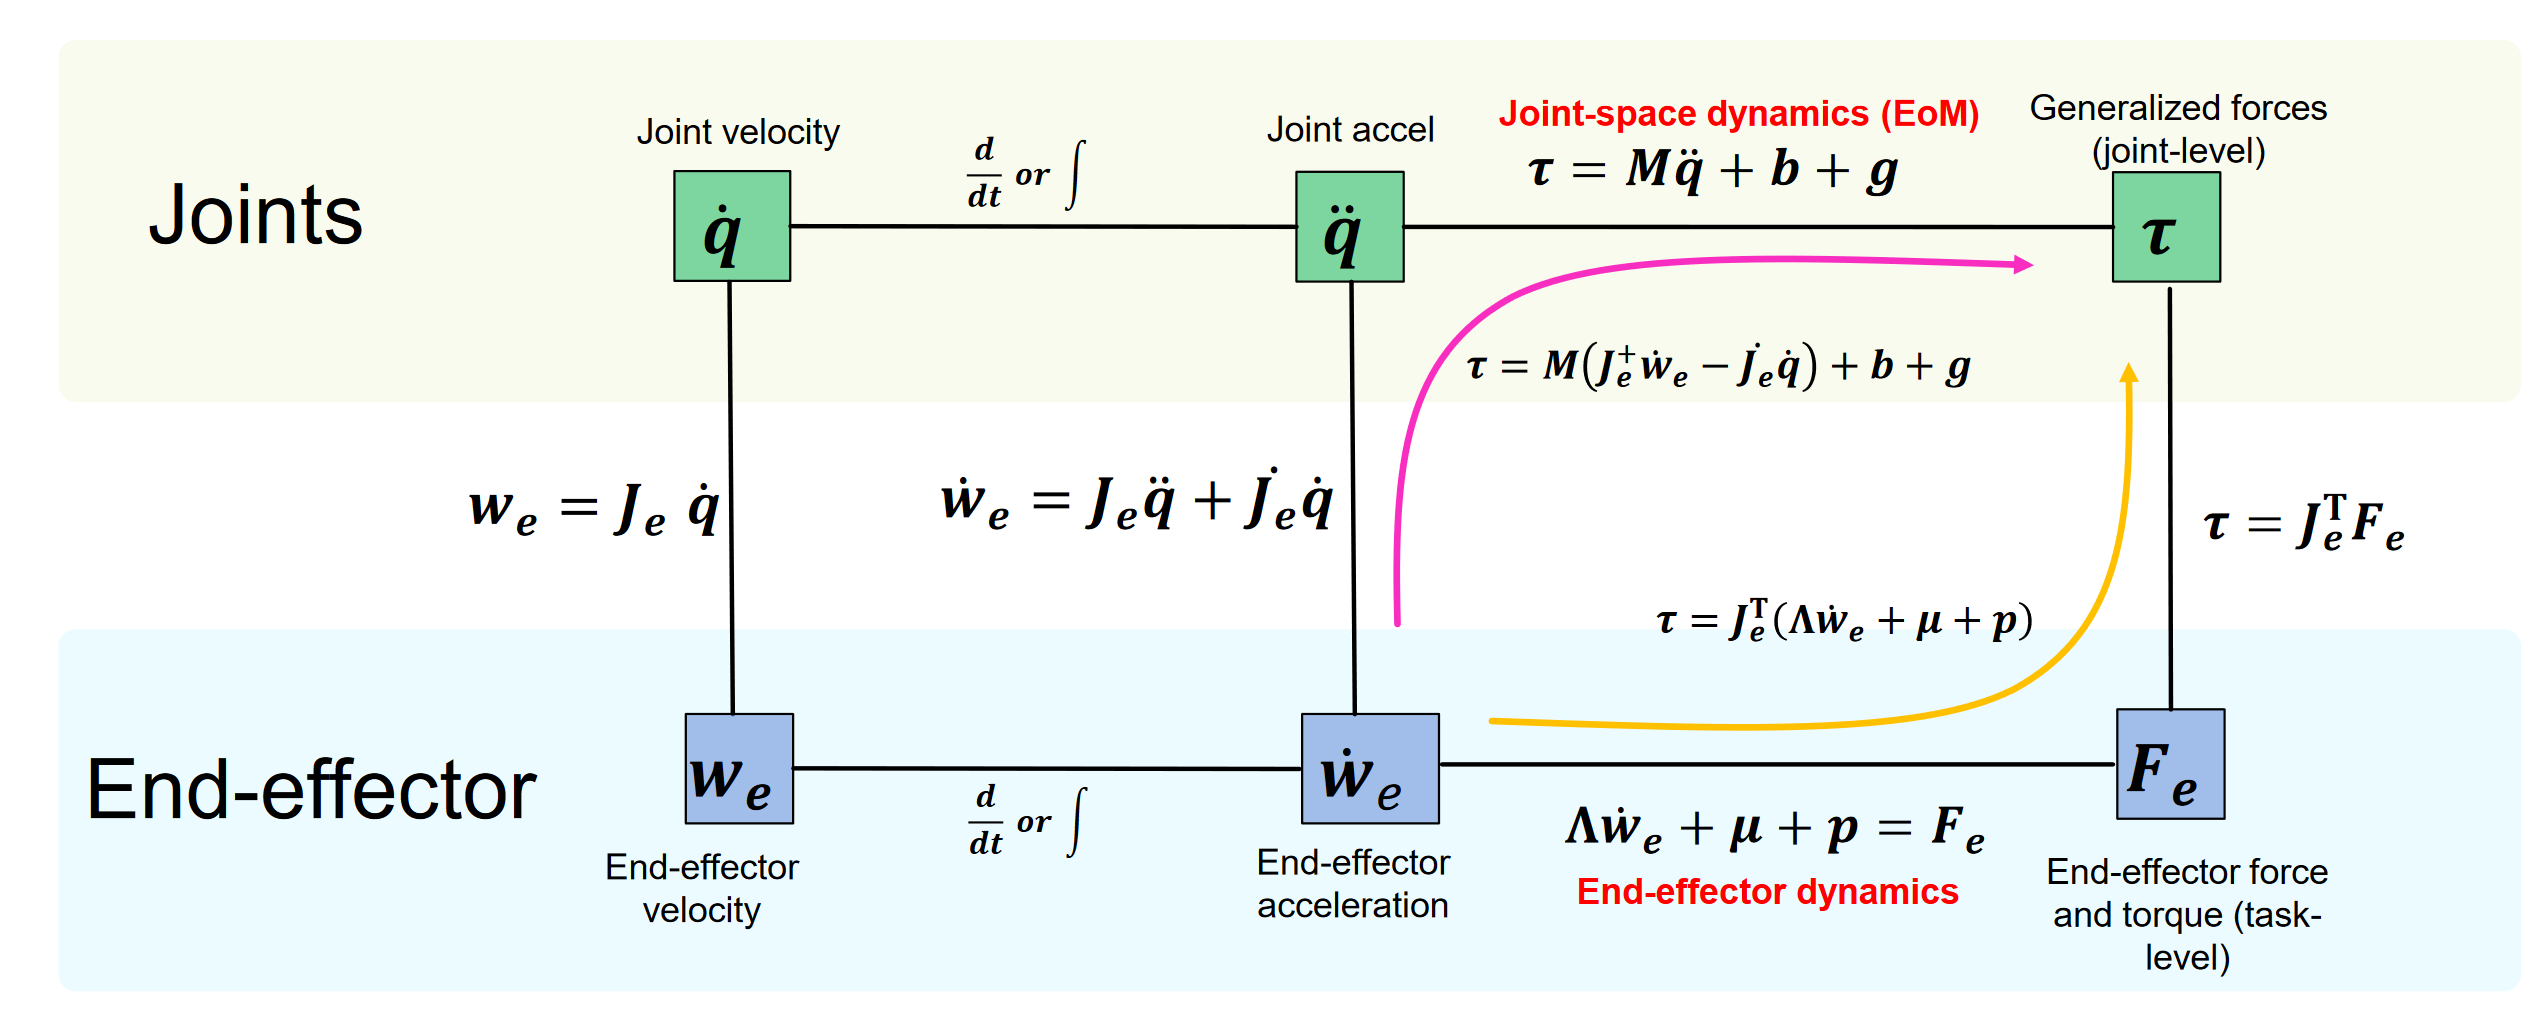
\includegraphics[width=\textwidth, trim={0cm 0cm 0cm 2cm},clip]{images/dynamics.png}

\begin{minipage}[c]{0.475\textwidth}
    \begin{itemize}\compresslist
    \item $\mathbf{g}(\mathbf{q})\in \mathbb{R}^{n_q}$: gravitational terms
    
    $\mathbf{g} = \sum_{i=1}^{n_b}-~_{\mathcal{A}}\mathbf{J}_{S_i}^\top ~_{\mathcal{A}}\mathbf{F}_{g,i}$ 
    \item $\tau\in \mathbb{R}^{n_\tau}$:  external generalized forces/torques
    
    $\tau = \sum_{k=1}^{n_A} \tau_{a,k}\tau_{ext}$
      \begin{itemize}[label=$\circ$]\compresslist
        \item actuator generalized force 
        
        \hspace{-12pt}$\tau_{a,k} = (\mathbf{J}_{S_k} - \mathbf{J}_{S_{k-1}})^\top\mathbf{F}_{a,k} + (\mathbf{J}_{R_k} - \mathbf{J}_{R_{k-1}})^\top \mathbf{T}_{a,k}$
        
        $\mathbf{T}$ is torque here
        \item external generalized force 
        
        \hspace{-12pt}$\tau_{ext} = \sum_{j=1}^{n_{f,ext}}\mathbf{J}_{P,j}^\top \mathbf{F}_j + \sum_{j=1}^{n_{m,ext}}\mathbf{J}_{R,j}^\top\mathbf{T}_{ext, j}$
      \end{itemize}
    \item $\mathbf{S}\in \mathbb{R}^{n_\tau\times n_q}$: selection matrix of actuated joints
 
\end{itemize}
\end{minipage}
\hfill
\begin{minipage}[c]{0.475\textwidth}
    \begin{itemize}\compresslist
           \item $\mathbf{F}_c\in \mathbb{R}^{n_c}$: external Cartesian forces 
    
    (e.g. from contacts)
      \begin{itemize}[label=$\circ$]\compresslist
        \item Soft Contact Model: $\mathbf{F}_c = k_p(\mathbf{r}_c - \mathbf{r}_{c0}) + k_d\dot{\mathbf{r}}_c$
        \item Contact Force from Constraint
        
        $\mathbf{r}_c = \text{const}\quad\dot{\mathbf{r}}=\ddot{\mathbf{r}}_c=0$
        
        \hspace{-20pt}$\mathbf{F}_c = (\mathbf{J}_c\mathbf{M}^{-1}\mathbf{J}_c^\top)^{-1}\left(\mathbf{J}_c\mathbf{M}^{-1}(\mathbf{S}^{\top}\tau-\mathbf{b}-\mathbf{g})+\dot{\mathbf{J}}_c\mathbf{u}\right)$
      \end{itemize}
    \item $\mathbf{J}_c(\mathbf{q})\in \mathbb{R}^{n_c\times n_q}$: Geometric Jacobian 
    
    corresponding to external force
    \item Kinect Energy: 
    
    $\mathcal{T}(\mathbf{q},\dot{\mathbf{q}}) = \frac{1}{2}\dot{\mathbf{q}}^\top\left(\sum_{i=1}^{n_b}(\mathbf{J}_{S_i}^\top m\mathbf{J}_{S_i} + \mathbf{J}_{R_i}^\top \Theta_{S_i}\mathbf{J}_{R_i})\right)\dot{\mathbf{q}}$
    \item Potential Energy: $\mathcal{U}_g = -\sum_{i=1}^{n_b} \mathbf{r}_{S_i}^\top \mathbf{F}_{g_i}$
    \end{itemize}
\end{minipage}

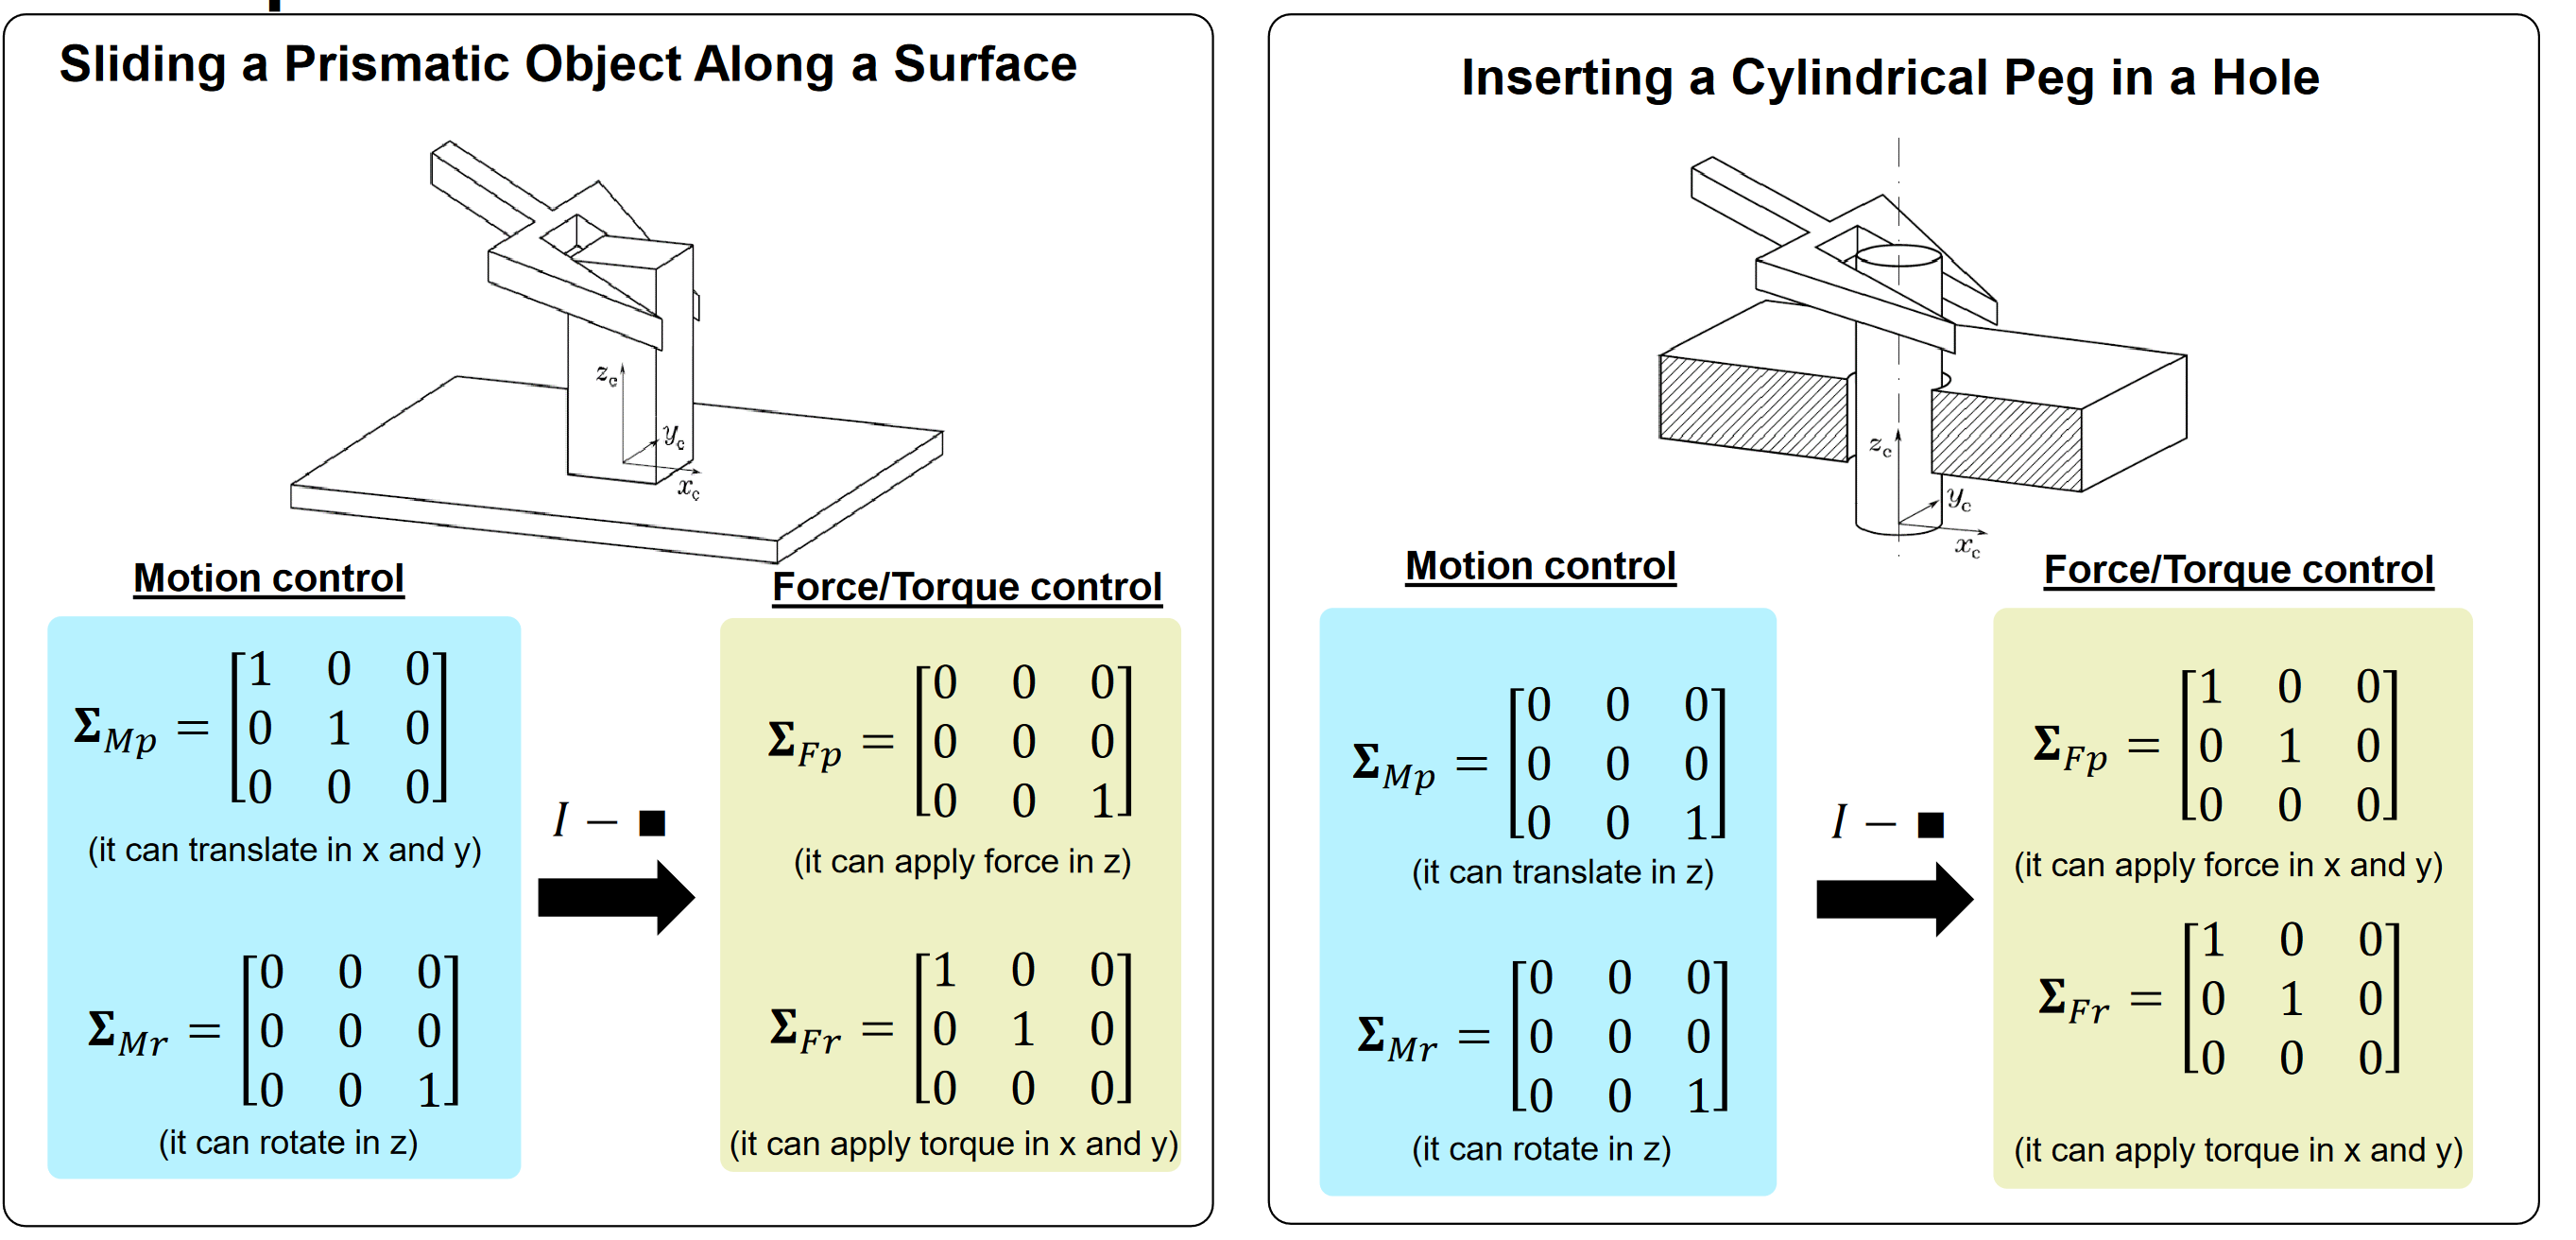
\includegraphics[width=\textwidth]{images/selection_matrix.png}


\colorbox[HTML]{CCFFFF}{\makebox[\textwidth-2\fboxsep][l]{\bf Dynamics of Floating Base System: }}
\begin{itemize}\compresslist
    \item \textit{Contact Force}
    \begin{itemize}[label=$\circ$]\compresslist
        \item Soft Contact : $\textbf F_c = k_p (\textbf r_c - \textbf  r_{c0}) + k_d \dot{\textbf r}_c$
        \item Constraint Contact : $\textbf r_c = \text{const}$ $\dot{\textbf r}_c =\textbf J_c\textbf u = \textbf 0 $ $ \ddot{\textbf r}_c = \textbf J_c \dot{\textbf u}+\dot{\textbf J}_c\textbf u =  \textbf 0$

        $\textbf F_c = (\textbf J_c\textbf M^{-1}\textbf J_c^\top)^{-1}\left(\textbf J_c\textbf  M^{-1}(\textbf S^\top \tau -\textbf b-\textbf g) +  \dot{\textbf J}_c \textbf u\right)$
    \end{itemize}
\end{itemize}





}


%----------------------------------------------------------------
%	Dynamics
%----------------------------------------------------------------
\headerbox{}{name=conclusion,column=3,span=1}{
\begin{itemize}\compresslist
    \item \textit{Constraint Consistent Dynamics}: 
    \begin{itemize}[label=$\circ$]\compresslist
        \item $\textbf N_c = \mathbb I - \textbf M^{-1}\textbf J_c^\top (\textbf J_c \textbf M^{-1}\textbf J_c^\top)^{-1} \textbf J_c$
        \item $\textbf  N_c^\top (\textbf  M\dot{\textbf u}+\textbf b+\textbf g) = \textbf  N_c^\top \textbf S^\top \tau$
    \end{itemize}

    \item \textit{Impulse Transfer}: 
    \begin{itemize}[label=$\circ$]\compresslist
        \item end-effector inertia : $\boldsymbol \Lambda_c  = (\textbf J_c\textbf M^{-1}\textbf J_c^\top)^{-1}$
        \item instantaneous change : 
        
        $\Delta u =\textbf  u^+-\textbf u^0= - \textbf M^{-1}\textbf J_c^\top (\textbf J_c\textbf M^{-1}\textbf J_c^\top)^{-1}\textbf J_c\textbf u^{-}$
        \item post-impact generalized velocity : 
        
        $\textbf u^+ = \textbf N_c \textbf u^{-1}$
        \item Energy Loss : $E_{loss} = -\frac{1}{2}\Delta \textbf u^\top_c\boldsymbol \Lambda_c \Delta \textbf u$
    \end{itemize}

  
\end{itemize}

\colorbox[HTML]{CCFFFF}{\makebox[\textwidth-2\fboxsep][l]{\bf Joint Space Dynamic Control: }}


\begin{itemize}\compresslist
    \item \textit{Gravity Compensation } : 
    
    $\tau^* = k_p(\textbf q^* - \textbf q) + k_d(\dot{\textbf q}^*-\dot{\textbf q})+\textbf g(\textbf q)$
    \item \textit{Inverse Dynamics Control} :
    
    $\ddot{\mathbf{q}}^* = k_p(\mathbf{q}^* - \mathbf{q}) + k_d(\dot{\mathbf{q}}^* - \dot{\mathbf{q}})$   ,  $\omega = \sqrt{k_p}~ D = \frac{k_d}{2\sqrt{k_p}}$
\end{itemize}

\colorbox[HTML]{CCFFFF}{\makebox[\textwidth-2\fboxsep][l]{\bf Task Space Dynamic Control: }}
 $$\dot{\mathbf{w}}_e = \begin{pmatrix}\ddot{\mathbf{r}}\\\dot{\boldsymbol{\omega}}\end{pmatrix} = \mathbf{J}_e\ddot{\mathbf{q}} + \dot{\mathbf{J}}_e\dot{\mathbf{q}}$$

\begin{itemize}\compresslist
    \item Multi-task Decomposition:
      \begin{itemize}[label=$\circ$]\compresslist
        \item Equal Priority: 
        
        $\ddot{\mathbf{q}} = \begin{bmatrix}\mathbf{J}_1\\\vdots\\\mathbf{J}_{n_t}\end{bmatrix}^+\left(\begin{pmatrix}\dot{\mathbf{w}}_1^*\\\vdots\\ \dot{\mathbf{w}}^*_{n_t}\end{pmatrix} - \begin{bmatrix}\dot{\mathbf{J}}_1\\\vdots\\\dot{\mathbf{J}}_{n_t}\end{bmatrix}\dot{\mathbf{q}}\right)$
        \item Prioritization: 
        
        $\ddot{\mathbf{q}} = \sum_{i=1}^{n_t}\mathbf{N}_{i}\ddot{\mathbf{q}}_i$ 
        
        $\ddot{\mathbf{q}}_i = (\mathbf{J}_i\mathbf{N}_{i})^+\left(\dot{\mathbf{w}}_i^* - \dot{\mathbf{J}}_i\dot{\mathbf{q}} - \mathbf{J}_i\sum_{k=1}^{i-1}\mathbf{N}_k\ddot{\mathbf{q}}_k\right)$ 
        
        $\mathbf{N}_i = \mathbb{I} - \mathbf{J}_i^+\mathbf{J}_i$ is the null space
      \end{itemize}
    \item End-effector Dynamics: $\Lambda_e \dot{\mathbf{w}}_e + \boldsymbol{\mu} + \mathbf{p} = \mathbf{F}_e$
      \begin{itemize}[label=$\circ$]\compresslist
        \item $\Lambda_e = (\mathbf{J}_e\mathbf{M}^{-1}\mathbf{J}_e^\top)^{-1}$: end-effector inertia
        \item $\boldsymbol{\mu} = \Lambda_e\mathbf{J}_e\mathbf{M}^{-1}\mathbf{b} - \Lambda_e \dot{\mathbf{J}}_e\dot{\mathbf{q}}$: end-effector centrifugal/Coriolis
        \item $\mathbf{p} = \Lambda_e \mathbf{J}_e\mathbf{M}^{-1}\mathbf{g}$: end-effector gravitational
        \item $\tau = \mathbf{J}_e^\top \mathbf{F}_e$ : joint torque 
      \end{itemize}

    \item End-effector Motion Control: 
    $$\begin{aligned}\tau^* &= \mathbf{J}^\top(\Lambda_e\dot{\mathbf{w}}_e^*+\boldsymbol{\mu} + \mathbf{p}) \\&= \mathbf{J}^\top \Lambda_e\dot{\mathbf{w}}_e^*+\mathbf{b}-\mathbf{J}^\top \Lambda_e\dot{\mathbf{J}}_e\dot{\mathbf{q}}+\mathbf{g}\end{aligned}$$
    \item Operational Space Control: 
    
    $\tau^* = \mathbf{J}^\top(\Lambda \mathbf{S}_M\dot{\mathbf{w}}_e + \mathbf{S}_F\mathbf{F}_c + \boldsymbol{\mu} +\mathbf{p})$
      
     $\Sigma_p =\begin{bmatrix}\sigma_{px}&0&0\\0&\sigma_{py}&0\\0&0&\sigma_{pz}\end{bmatrix}$, $\Sigma_r = \begin{bmatrix}\sigma_{rx}&0&0\\0&\sigma_{ry}&0\\0&0&\sigma_{rz}\end{bmatrix}$ 
        
    $\sigma_i=1$ if the axis is free of motion, otherwise $0$
    

\end{itemize}




}




\end{poster}
\newpage

\begin{poster}
{
headerborder=closed, % Adds a border around the header of content boxes
colspacing=0.4em, % Column spacing
bgColorOne=white, % Background color for the gradient on the left side of the poster
bgColorTwo=white, % Background color for the gradient on the right side of the poster
borderColor=chipurple, % Border color
headerColorOne=chiorange, % Background color for the header in the content boxes (left side)
headerColorTwo=chipurple, % Background color for the header in the content boxes (right side)
headerFontColor=white, % Text color for the header text in the content boxes
boxColorOne=white, % Background color of the content boxes
textborder=roundedleft, % Format of the border around content boxes, can be: none, bars, coils, triangles, rectangle, rounded, roundedsmall, roundedright or faded
eyecatcher=true, % Set to false for ignoring the left logo in the title and move the title left
headerheight=0.0\textheight, % Height of the header
headershape=roundedright, % Specify the rounded corner in the content box headers, can be: rectangle, small-rounded, roundedright, roundedleft or rounded
headerfont=\Large\bf\textsc, % Large, bold and sans serif font in the headers of content boxes
%textfont={\setlength{\parindent}{1.5em}}, % Uncomment for paragraph indentation
linewidth=2pt % Width of the border lines around content boxes
}
%----------------------------------------------------------------
%	TITLE SECTION 
%----------------------------------------------------------------
{} % Poster title
{}


%----------------------------------------------------------------
%	Dynamics
%----------------------------------------------------------------
\headerbox{}{name=conclusion,column=0,span=1}{
     $\mathbf{S}_M\!=\!\begin{bmatrix}\mathbf{C}^\top \Sigma_p\mathbf{C}&0\\0&\mathbf{C}^\top \Sigma_r \mathbf{C}\end{bmatrix}$
     
     $\mathbf{S}_F\!=\!\begin{bmatrix}\mathbf{C}^\top (\mathbb{I} -\Sigma_p)\mathbf{C}&0 \\ 0& \mathbf{C}^\top (\mathbb{I}-\Sigma_r)\mathbf{C}\end{bmatrix}$


    
\colorbox[HTML]{CCFFFF}{\makebox[\textwidth-2\fboxsep][l]{\bf Inverse Dynamics for Floating-Base Systems: }}


\begin{itemize}\compresslist
    \item Hierarchical Least Square Optimization: 

    $\underset{\mathbf{x}}{\text{min}}\Vert \mathbf{A}_i\mathbf{x} - \mathbf{b}_i\Vert_2$ with priority

    normally $\textbf x = \begin{bmatrix}\ddot {\textbf q}^\top &\boldsymbol\tau^\top & _{\mathcal I}\textbf F_E^\top\end{bmatrix}^\top$
      \begin{enumerate}\compresslist
        \item $n_T$: number of tasks
        \item $\mathbf{x} = \mathbf{0}$: initial optimal solution
        \item $\mathbf{N}_1 = \mathbb{I}$: initial null-space projector
        \item for $i=1 \to n_T$ do
          \begin{enumerate}\compresslist
            \item $\mathbf{x}_i \gets (\mathbf{A}_i\mathbf{N}_i)^+(\mathbf{b}_i-\mathbf{A}_i\mathbf{x})$
            \item $\mathbf{x} \gets \mathbf{x} +  \mathbf{N}_i\mathbf{x}_i$
            \item $\mathbf{N}_{i+1} = \mathcal{N}(\left[\mathbf{A}_1^\top \cdots \mathbf{A}_i^\top\right]^\top)$: null-space
            
            \hspace{-10pt}normally $\mathcal{N}(\mathbf{A}) = \mathbb{I} - \mathbf{A}^+ \mathbf{A}$, $\mathcal{N}(\mathbf{A})\mathbf{A} = \mathbf{0}$
          \end{enumerate}
      \end{enumerate}
\end{itemize}

}

%----------------------------------------------------------------
%	Legged Robot
%----------------------------------------------------------------
\headerbox{Legged Robot}{name=conclusion,column=0,span=1,row=0.4}{

\textbf{Input} : $\mathbf{q}, \dot{\mathbf{q}}$

\textbf{Optimization Target} : $\ddot{\mathbf{q}}, \mathbf{F}_c, \boldsymbol{\tau}$

\textbf{Tasks}:

\begin{itemize}
    \item Equation of Motion: $\begin{bmatrix}\mathbf{M}(\mathbf{q}) & -\mathbf{J}_c & -\mathbf{S}^\top\end{bmatrix}\begin{bmatrix}\ddot{\mathbf{q}} \\ \mathbf{F}_c \\ \boldsymbol{\tau}\end{bmatrix} = -\mathbf{b}(\dot{\mathbf{q}},\mathbf{q}) - \mathbf{g}(\mathbf{q})$
    \item End Effector Desired Velocity $\mathbf{w}^*_e$: $\begin{bmatrix}\mathbf{J}_e & \mathbf{0} & \mathbf{0}\end{bmatrix}\begin{bmatrix}\ddot{\mathbf{q}} \\ \mathbf{F}_c \\ \boldsymbol{\tau}\end{bmatrix} = \dot{\mathbf{w}}_e - \dot{\mathbf{J}}_c \dot{\mathbf{q}}$ where $\dot{\mathbf{w}}_e = k_p(\mathbf{r}_e^* - \mathbf{r}_e) - k_d(\mathbf{w}_e^* - \mathbf{w}_e)$
    \item Torque minimize: $\begin{bmatrix}\mathbf{0} & \mathbf{0} & \mathbb{I}\end{bmatrix}\begin{bmatrix}\ddot{\mathbf{q}} \\ \mathbf{F}_c \\ \boldsymbol{\tau}\end{bmatrix} = \mathbf{0}$
    \item Torque limits: $\begin{bmatrix}\mathbf{0} & \mathbf{0} & \mathbb{I}\end{bmatrix}\begin{bmatrix}\ddot{\mathbf{q}} \\ \mathbf{F}_c \\ \boldsymbol{\tau}\end{bmatrix} \le \mathbf{1} \cdot \tau_{\text{max}}$ and $\begin{bmatrix}\mathbf{0} & \mathbf{0} & -\mathbb{I}\end{bmatrix}\begin{bmatrix}\ddot{\mathbf{q}} \\ \mathbf{F}_c \\ \boldsymbol{\tau}\end{bmatrix} \le -\mathbf{1} \cdot \tau_{\text{max}}$
   
    \item Contact Force minimize: 
        \[
        \begin{bmatrix}\mathbf{0} & \mathbb{I} & \mathbf{0}\end{bmatrix}\begin{bmatrix}\ddot{\mathbf{q}} \\ \mathbf{F}_c \\ \boldsymbol{\tau}\end{bmatrix} = \mathbf{0}
        \]
    \item Friction Cone: 
    
    $\begin{bmatrix}\begin{bmatrix}0 & -1 \\ 1 - \mu & -1 - \mu\end{bmatrix} & \mathbf{0} \\ \mathbf{0} & \begin{bmatrix}0 & -1 \\ 1 - \mu & -1 - \mu\end{bmatrix}\end{bmatrix}  \mathbf{F}_c  \le \mathbf{0}$ 
    
    for $2D$ $x-z$ problem
\end{itemize}

\textbf{Optimization}

\textit{[HO] Hierarchical Least Square Optimization}




}

%----------------------------------------------------------------
%	RotorCraft
%----------------------------------------------------------------
\headerbox{RotorCraft}{name=conclusion,column=1,span=1, row=0}{
\centering
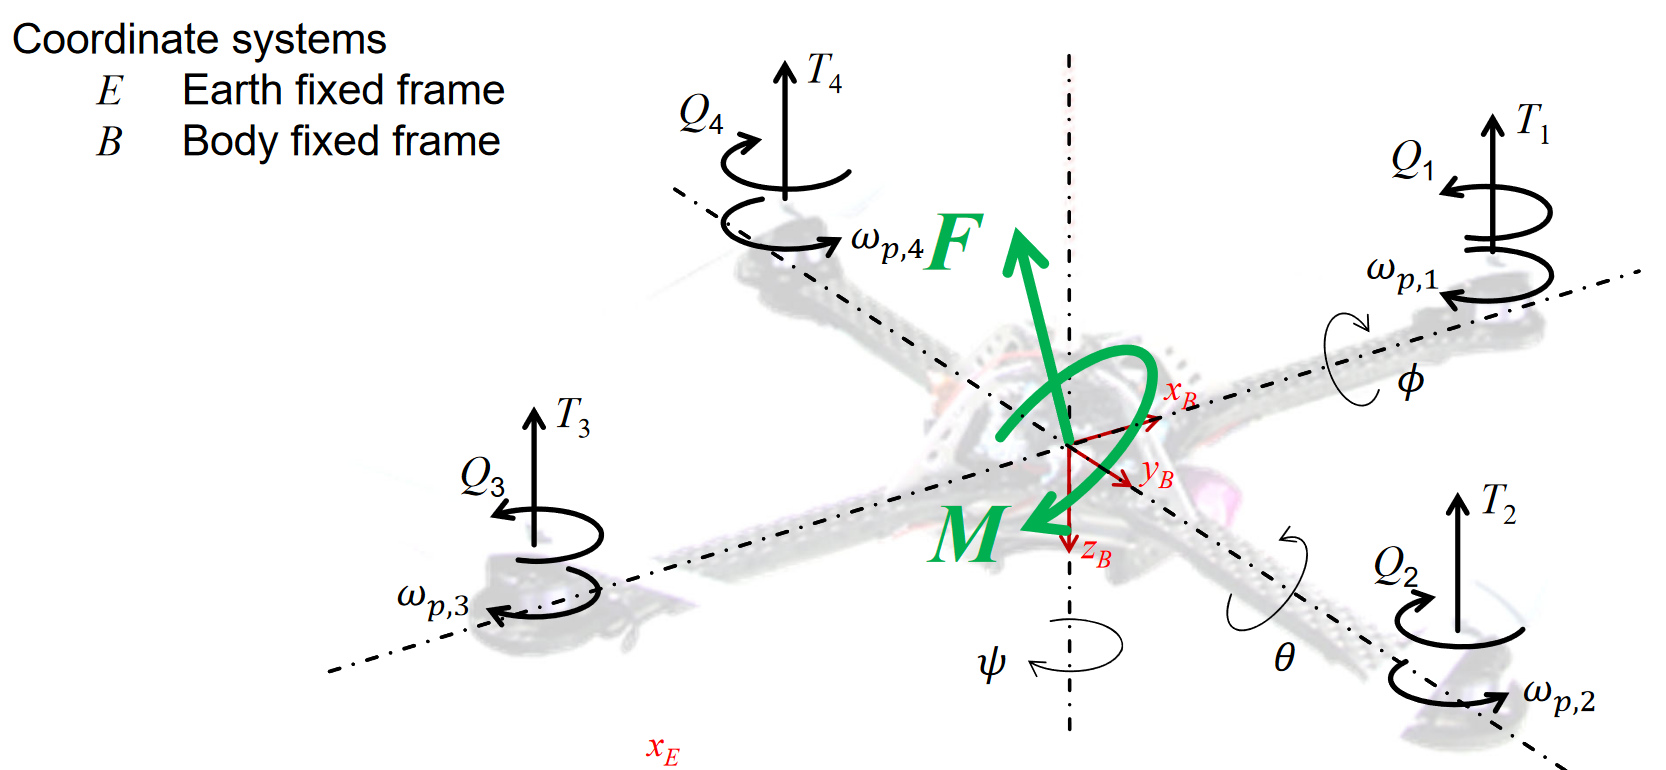
\includegraphics[width=0.9\textwidth]{images/quadrotor_force.png}
\[
\underbrace{\begin{bmatrix}m\mathbb{I} &  0 \\ 0 & \boldsymbol{\Theta}\end{bmatrix}}_{\mathbf{M}}\underbrace{\begin{bmatrix}\dot{\boldsymbol{\nu}} \\ \dot{\boldsymbol{\omega}}\end{bmatrix}}_{\ddot{\mathbf{q}}} + \underbrace{\begin{bmatrix}\boldsymbol{\omega} \times m \boldsymbol{\nu} \\ \boldsymbol{\omega} \times \boldsymbol{\Theta}\boldsymbol{\omega}\end{bmatrix}}_{\mathbf{b}} = \underbrace{\begin{bmatrix}\mathbf{F}\\\underbrace{M}_{\text{torque}}\end{bmatrix}}_{\boldsymbol{\tau}}
\]
$$
_{\mathcal{B}}\mathbf{F} = \underbrace{\mathbf{C}_{\mathcal{IB}}^\top ~_{\mathcal{I}}\begin{bmatrix}0\\0\\mg\end{bmatrix}}_{_{\mathcal{B}}\mathbf{F}_G} + 
\underbrace{\sum_{i=1}^4 ~_{\mathcal{B}}\begin{bmatrix}0\\0\\-T_i\end{bmatrix}}_{_{\mathcal{B}}\mathbf{F}_{\text{Aero}}}
$$
\[
_{\mathcal{B}}M = \underbrace{_{\mathcal{B}}\begin{bmatrix}l(T_4-T_2)\\l(T_1-T_3)\\0\end{bmatrix}}_{_{\mathcal{B}}M_T} + \underbrace{_{\mathcal{B}}\begin{bmatrix}0\\0\\ \sum_{i=1}^4 Q_i(-1)^i\end{bmatrix}}_{_{\mathcal{B}}Q}
\]

\begin{itemize}\compresslist
    \item $T_i$: Thrust force for propeller $i$, $T_i = b\omega_{p,i}^2$ generate lift for keeping the rotorcraft in the air
    \item $Q_i$: Drag force of propeller $i$, $Q_i = d\omega_{p,i}^2$ rotor drag
    \item $_{\mathcal{B}}M_T$: Thrust Induced moment 
    
    $M_T = \begin{bmatrix}-\sin\theta\\\sin\phi\cos\theta\\\cos\phi \cos\theta\end{bmatrix}mg$
    
    
\end{itemize}


\begin{itemize}\compresslist
     \item $_{\mathcal{B}}Q$: Drag torques
    \item $\mathbf{C}_{\mathcal{IB}}$: transition from earth frame to body frame
    \item $_{\mathcal{B}}\boldsymbol{\omega}$: Body Angular Velocity 
    
    $_{\mathcal{B}}\boldsymbol{\omega} =_{\mathcal{B}} \begin{bmatrix}p\\q\\r\end{bmatrix} = \begin{bmatrix}\dot{\phi}\\\dot{\theta}\\\dot{\psi}\end{bmatrix}$
    \item $\omega_{p,i}$: Rotational Speed of Propeller $i$
    \item $_{\mathcal{B}}\boldsymbol{\nu}$: Basis Translation Velocity 
    
    $_{\mathcal{B}}\boldsymbol{\nu} = _{\mathcal{B}}\begin{bmatrix}u\\v\\w\end{bmatrix} = _{\mathcal{B}}\begin{bmatrix}\dot{x}\\\dot{y}\\\dot{z}\end{bmatrix}$
    \item $l$: Distance of the propeller from the central of gravity
\end{itemize}

\colorbox[HTML]{CCFFFF}{\makebox[\textwidth-2\fboxsep][l]{\bf Control of Quadrotor: }}
\[
\begin{array}{lr}
    \boldsymbol{\Theta}_{xx}\dot{p} = q \cdot r(\boldsymbol{\Theta}_{yy} - \boldsymbol{\Theta}_{zz}) + U_2 & (1) \\
    \boldsymbol{\Theta}_{yy}\dot{q} = r \cdot p(\boldsymbol{\Theta}_{zz} - \boldsymbol{\Theta}_{xx}) + U_3 & (2) \\
    \boldsymbol{\Theta}_{zz}\dot{r} = U_4 & (3) \\
    m\dot{u} = m(r \cdot v - q \cdot w) - \sin\theta~ mg & (4) \\
    m\dot{v} = m(p \cdot w - r \cdot u) + \sin\phi \cos\theta ~ mg & (5) \\
    m\dot{w} = m(q \cdot u - p \cdot v) + \cos\phi \cos\theta ~ mg - U_1 & (6)
\end{array}
\]




}







% ----------------------------------------------------------------
%	RotorCraft
%----------------------------------------------------------------
\headerbox{}{name=conclusion,column=2,span=1}{

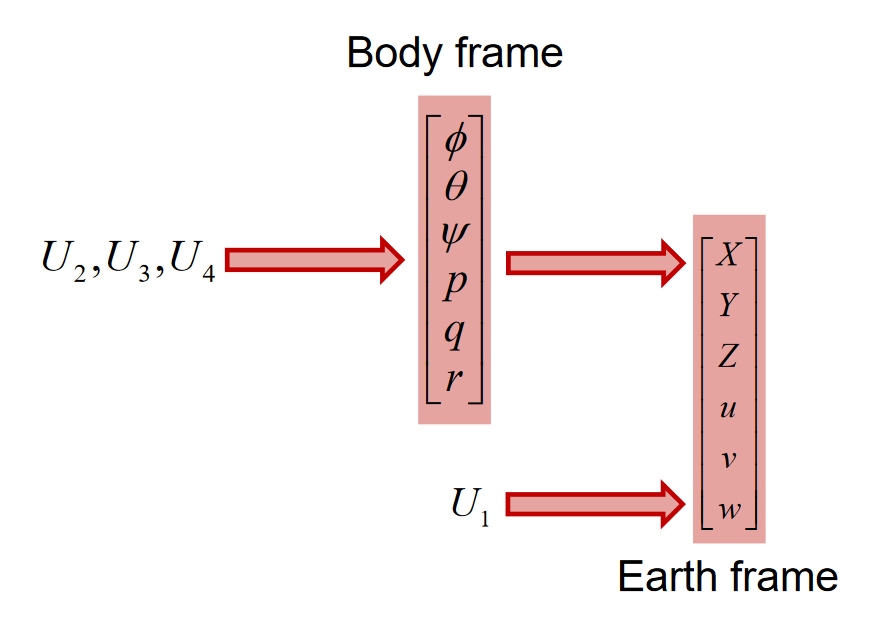
\includegraphics[width=0.8\textwidth,trim={0cm 0cm 0cm 0cm},clip]{images/rotorcraft_hierarchicachy_control.png}
\vspace{-10pt}
\[
\begin{bmatrix}U_1\\U_2\\U_3\\U_4\end{bmatrix} = 
\underbrace{\begin{bmatrix}b & b & b & b\\
0 & -lb & 0 & lb\\
lb & 0 & -lb & 0\\
-d & d & -d & d\end{bmatrix}}_{\mathbf{A}}
\begin{bmatrix}\omega_{p,1}^2\\\omega_{p,2}^2\\\omega_{p,3}^2\\\omega_{p,4}^2\end{bmatrix}
\]
\vspace{-20pt}
\begin{itemize}\compresslist
    \item \textit{Equilibrium}
$_{\mathcal{B}}\boldsymbol{\nu} = \phi = \theta = \mathbf{0}$
  
       $_{\mathcal{B}} \dot{\boldsymbol{\omega}} = \boldsymbol{\Theta}^{-1}\begin{bmatrix}U_2 & U_3 & U_4\end{bmatrix}^\top$
       
      $
      \begin{array}{l}
          U_1 = T^* \\
          U_2 = (\phi^* - \phi)k_{p,\text{roll}} - \dot{\phi} k_{d,\text{roll}} \\
          U_3 = (\theta^* - \theta)k_{p,\text{pitch}} - \dot{\theta} k_{d,\text{pitch}} \\
          U_4 = (\psi^* - \psi)k_{p,\text{yaw}} - \dot{\psi} k_{d,\text{yaw}}
      \end{array}
      $


\item \textit{Altitude Control} $x = y = u = v = 0$
  \begin{itemize}[label=$\circ$]\compresslist
      \item $\dot{w} = g - \frac{1}{m}\underbrace{\cos\phi \cos\theta ~ U_1}_{T_z}$
      \item $T_z = -k_p(z^* - z) + k_d \dot{z} - mg$
  \end{itemize}

\item \textit{Position Control}
  \begin{itemize}[label=$\circ$]\compresslist
      \item $_{\mathcal{B}}{\dot{\boldsymbol{\nu}}} = \frac{1}{m}\begin{bmatrix}T_x & T_y & T_z\end{bmatrix}^\top + \begin{bmatrix}0 & 0 & g\end{bmatrix}^\top$
  \end{itemize}

\end{itemize}



\colorbox[HTML]{CCFFFF}{\makebox[\textwidth-2\fboxsep][l]{\bf Hexacopter: }}
$
\mathbf{A} = \begin{pmatrix}b & b & b & b & b & b\\ bl\sin_{30} & bl & bl\sin_{30} & -bl\sin_{30} & -bl & -bl\sin_{30}\\ -bl\cos_{30} & 0 & bl\cos_{30} & bl\cos_{30} & 0 & -bl\cos_{30} \\ d & -d & d & -d & d & -d\end{pmatrix}
$

\colorbox[HTML]{CCFFFF}{\makebox[\textwidth-2\fboxsep][l]{\bf MAV Control: }}
\begin{enumerate}\compresslist
    \item $_{\mathcal{B}}\boldsymbol{\omega}_{\text{ref}} = \text{PID}(_{\mathcal{B}}\boldsymbol{\nu}_{\text{ref}}, _{\mathcal{B}}\boldsymbol{\nu})$
    \item $U_1 = mg \\ \begin{bmatrix}U_2, U_3, U_4\end{bmatrix}^\top = \text{PID}(_{\mathcal{B}}\boldsymbol{\omega}_{\text{ref}}, ~_{\mathcal{B}}\boldsymbol{\omega}, ~_{\mathcal{B}}\dot{\boldsymbol{\omega}})$
    \item $\omega_p^2 = \mathbf{A}^+ \begin{bmatrix}U_1 & U_2 & U_3 & U_4\end{bmatrix}^\top$
\end{enumerate}

\colorbox[HTML]{CCFFFF}{\makebox[\textwidth-2\fboxsep][l]{\bf Propeller Aerodynamics: }}
\begin{minipage}[c]{0.275\textwidth}
    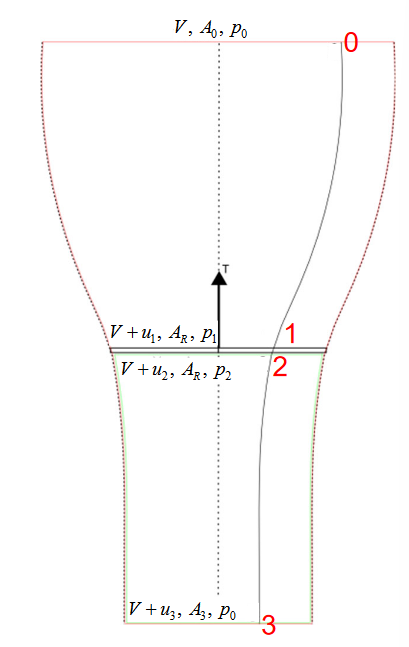
\includegraphics[width=\textwidth]{images/propeller.png}
\end{minipage}
\hfill
\begin{minipage}[c]{0.7\textwidth}
    \begin{itemize}\compresslist
    \item $u_1 = u_2$: no change of speed across rotor/propeller disc
    \item $\rho A_0 V = \rho A_R(V + u_1) = \rho A_R(V + u_2) = \rho A_3 u_3$: change in pressure
    \item $u_3 = 2u_1$: far wake slipstream velocity is twice the induced velocity
    \item $F_{\text{Thrust}} = \rho A_R(V + u_1)u_1$
    \item $P_{\text{Thrust}}\!=\!\frac{1}{2}\rho A_R(V\!+\!u_1)(2V\!+\!u_3) u_3$
    \item \textit{Hover case}: $P = \frac{F^{3/2}_{\text{Thrust}}}{\sqrt{2\rho A_R}} = \frac{(mg)^{3/2}}{\sqrt{2\rho A_R}}$
\end{itemize}
\end{minipage}



}


% ----------------------------------------------------------------
%	RotorCraft
%----------------------------------------------------------------
\headerbox{}{name=conclusion,column=3,span=1}{
\colorbox[HTML]{CCFFFF}{\makebox[\textwidth-2\fboxsep][l]{\bf [BEMT]Blade Elemental and Momentum Theory: }}
calculate forces for each element and sum them up
\centering
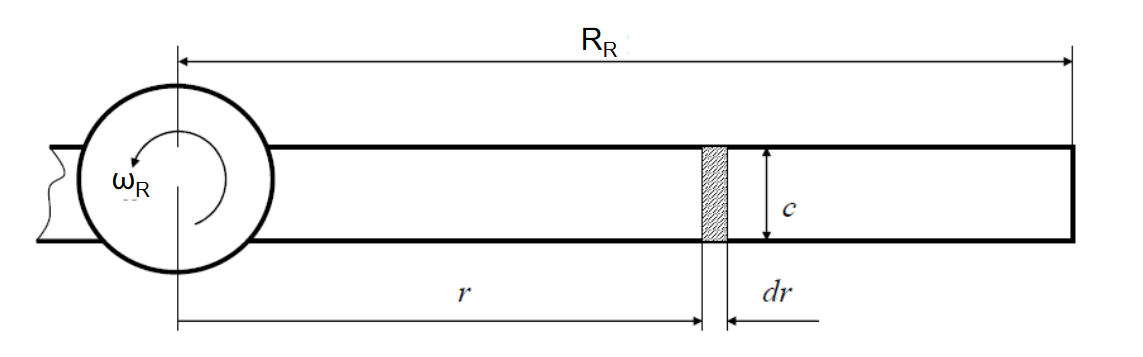
\includegraphics[width=0.9\textwidth]{images/BEMT_overview.png}

}

%----------------------------------------------------------------
%	Fixed Wing
%----------------------------------------------------------------
\headerbox{Fixed Wing}{name=conclusion,column=3,span=1,row=0.2}{

\centering
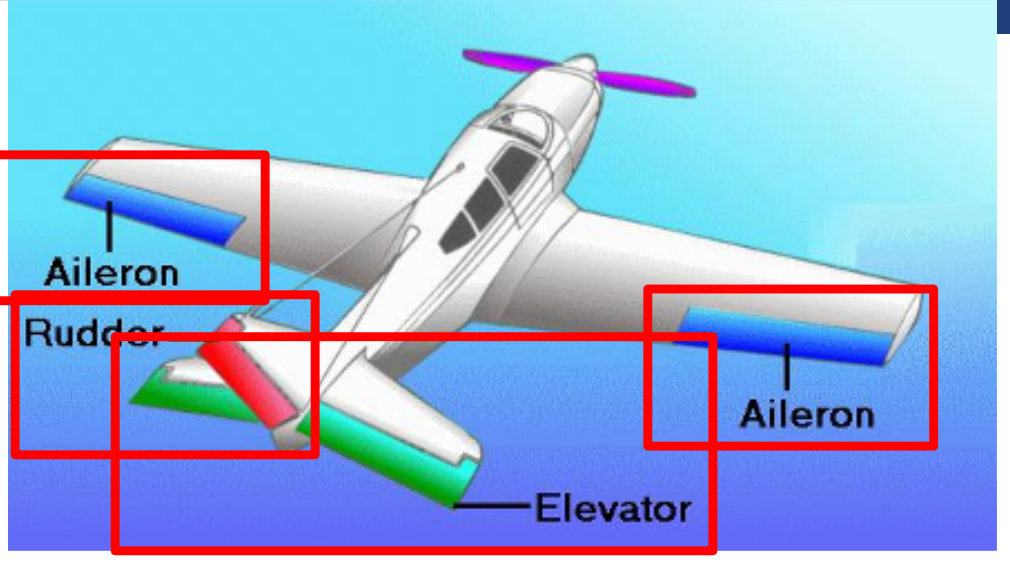
\includegraphics[width=0.9\textwidth]{images/control_surface.png}

\begin{itemize}\compresslist
    \item  Ailerons (rolling)
    \item Elevator (pitching)
    \item Rudder (yawing)
\end{itemize}

\centering
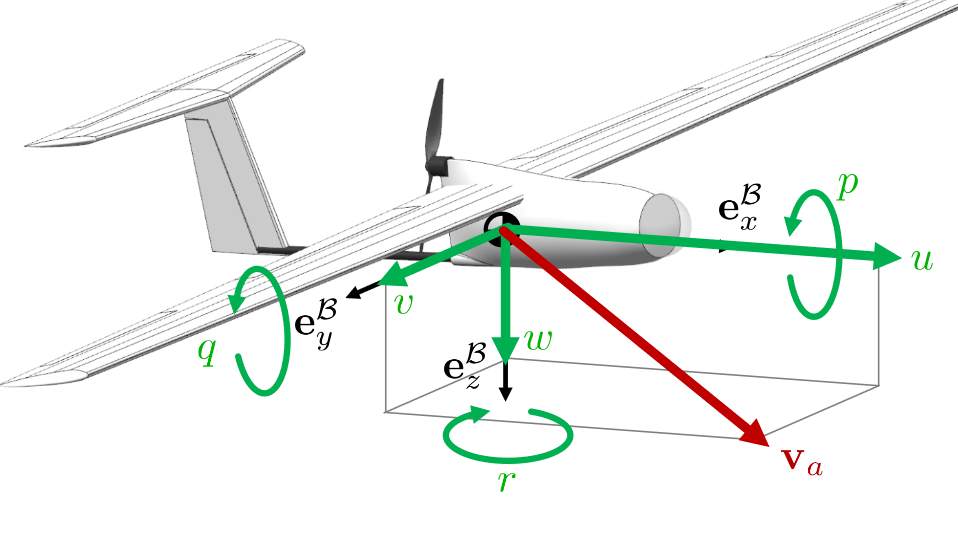
\includegraphics[width=0.9\textwidth,trim={0cm 2cm 0cm 2cm},clip]{images/fixed_wing_main_view.png}

\centering
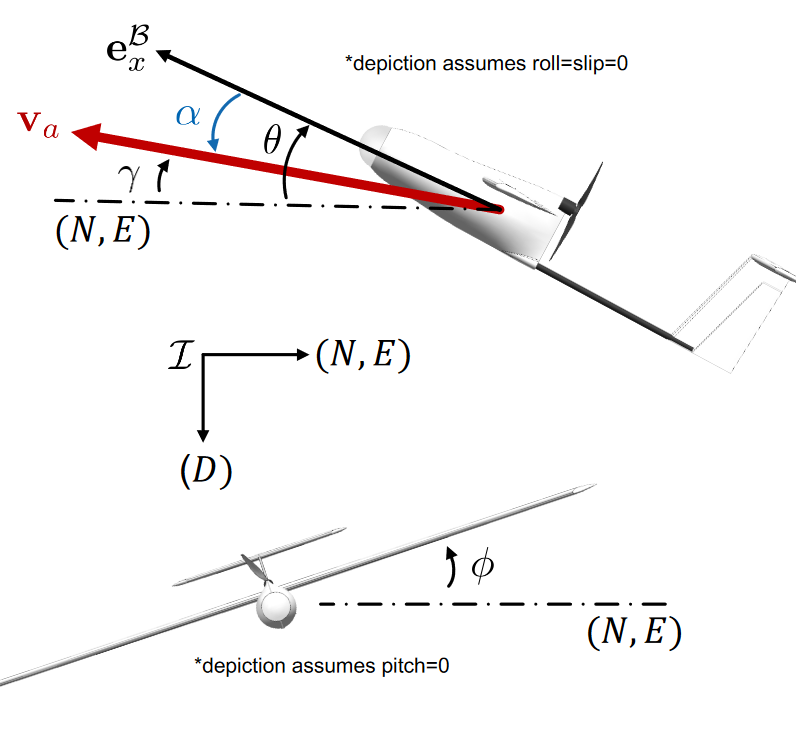
\includegraphics[width=0.9\textwidth]{images/fixed_wing_front_side_view.png}



}





\end{poster}
\newpage


\begin{poster}
{
headerborder=closed, % Adds a border around the header of content boxes
colspacing=0.4em, % Column spacing
bgColorOne=white, % Background color for the gradient on the left side of the poster
bgColorTwo=white, % Background color for the gradient on the right side of the poster
borderColor=chipurple, % Border color
headerColorOne=chiorange, % Background color for the header in the content boxes (left side)
headerColorTwo=chipurple, % Background color for the header in the content boxes (right side)
headerFontColor=white, % Text color for the header text in the content boxes
boxColorOne=white, % Background color of the content boxes
textborder=roundedleft, % Format of the border around content boxes, can be: none, bars, coils, triangles, rectangle, rounded, roundedsmall, roundedright or faded
eyecatcher=true, % Set to false for ignoring the left logo in the title and move the title left
headerheight=0.0\textheight, % Height of the header
headershape=roundedright, % Specify the rounded corner in the content box headers, can be: rectangle, small-rounded, roundedright, roundedleft or rounded
headerfont=\Large\bf\textsc, % Large, bold and sans serif font in the headers of content boxes
%textfont={\setlength{\parindent}{1.5em}}, % Uncomment for paragraph indentation
linewidth=2pt % Width of the border lines around content boxes
}
%----------------------------------------------------------------
%	TITLE SECTION 
%----------------------------------------------------------------
{} % Poster title
{}


%----------------------------------------------------------------
%	Fixed Wing
%----------------------------------------------------------------
\headerbox{}{name=conclusion,column=0,span=1}{
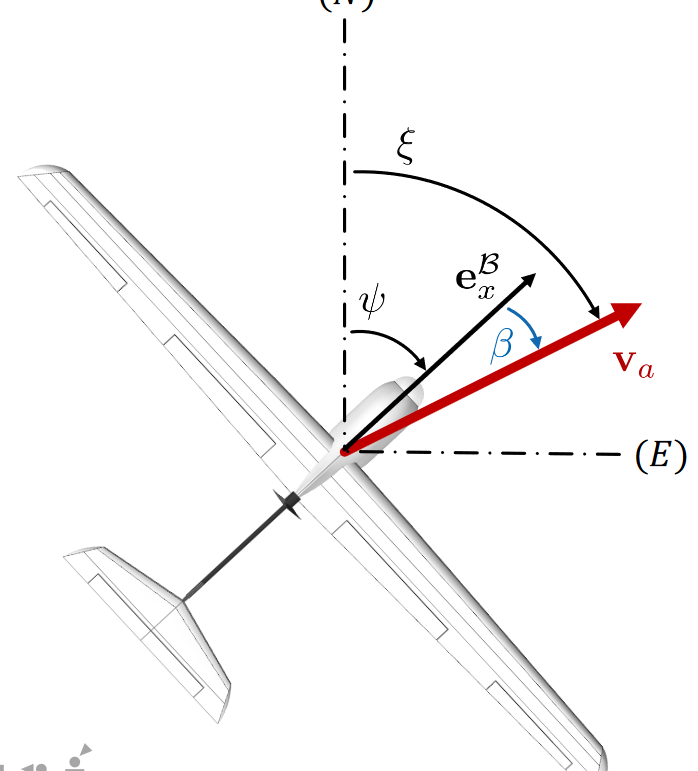
\includegraphics[width=0.9\textwidth,trim={0cm 4cm 0cm 6cm},clip]{images/fixed_wing_top_view.png}


\begin{itemize}
    \item $\alpha$: angle of attack $\atan(w/u)$
    
    \textit{stall} : $\begin{cases}\alpha\uparrow \to c_L\uparrow & \alpha <\text{stall} \\ \alpha^\uparrow  \to c_L\downarrow & \alpha > \text{stall}\end{cases}$ stall is not safe
    \item $\beta$: sideslip angle $\beta = \asin(v/V)$
    \item $\theta$: pitch angle
    \item $\phi$: roll angle, rotate about $x$-axis
    \item $\psi$: yaw angle
    \item $\gamma$: flight path angle, defined from horizon to $\mathbf{v}_a$
    \item $\xi$: heading angle, defined from North to $\mathbf{v}_a$
    \item $\mathbf{v}_w$: wind velocity
    \item $\mathbf{v}$: ground-based inertial velocity
    \item $L$: Lift $L=\frac{1}{2}\rho V^2 S{c_L}(\alpha)$, $S$ is the surface area
    \item $D$: Drag $D=\frac{1}{2}\rho V^2 S{c_D}$, perpendicular to Lift, parallel to air velocity $\mathbf{v}_a$
    \begin{itemize}[label=$\circ$]\compresslist
        \item minimum fuel for straight : $\underset{\alpha}{\text{argmax}}\frac{c_L(\alpha)}{c_D(\alpha)}$
        \item minimum fuel for circle : $\underset{\alpha}{\text{argmax}}\frac{c_L(\alpha)^3}{c_D(\alpha)^2}$
    \end{itemize}
    \item $L_m$: rolling moment $L_m = \frac{1}{2}\rho V^2 S{bc_l}$, 
    
    $b$ is the span of the wing
    \item $M_m$: pitching moment $M_m = \frac{1}{2}\rho V^2 S{\bar cc_m}$, 
    
    $\bar c$ is the average chord of the wing
    \item $N_m$: yawing moment $N_m = \frac{1}{2}\rho V^2 S{bc_n}$
\end{itemize}

\begin{minipage}[c]{0.475\textwidth}
    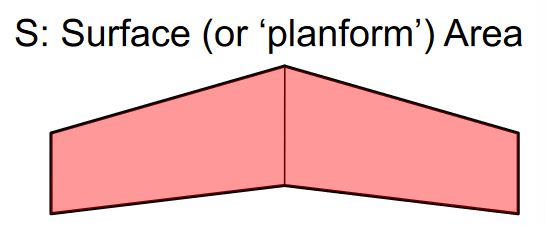
\includegraphics[width=\textwidth]{images/fixed_wing_surface.png}
\end{minipage}
\hfill
\begin{minipage}[c]{0.475\textwidth}
    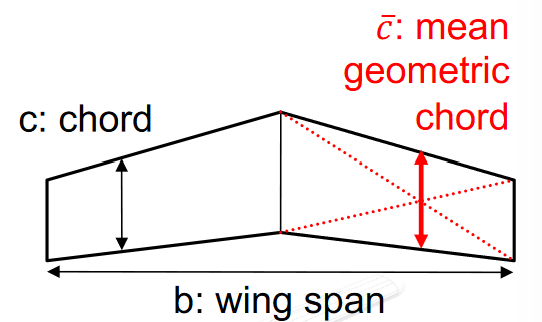
\includegraphics[width=\textwidth]{images/fixed_wing_parameter.png}
\end{minipage}

}


%----------------------------------------------------------------
%	Fixed Wing
%----------------------------------------------------------------
\headerbox{}{name=conclusion,column=1,span=1}{

\colorbox[HTML]{CCFFFF}{\makebox[\textwidth-2\fboxsep][l]{\bf Steady Level Turning Flight: }}


\centering
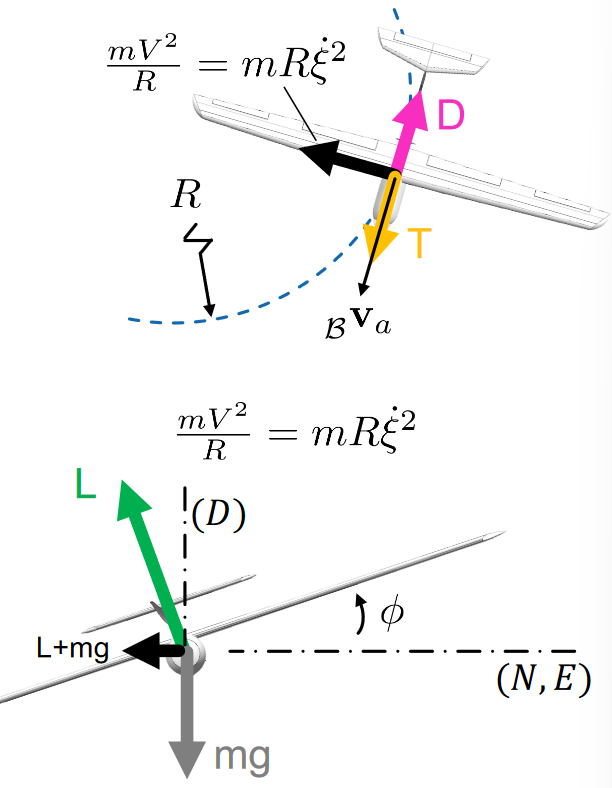
\includegraphics[width=0.7\textwidth,trim={0cm 2cm 0cm 0cm},clip]{images/fixed_wing_turning.png}


\begin{itemize}
    \item steady : $_{\mathcal B}\dot{\textbf v}_a = ~_{\mathcal B}\dot{\omega}=0$
    \item level : $\gamma = 0$
    \item turning : $\phi = \text{const}$ 
\end{itemize}
$
\begin{array}{l}
L\cos\phi = mg \\
L\sin\phi = m\frac{V^2}{R} = mR\dot{\xi} \\
D = T
\end{array}
\quad \rightarrow \quad
\begin{array}{l}
\dot{\xi} = \frac{g\tan\phi}{V} \\
L \propto \frac{1}{\cos\phi} \\
V \propto \sqrt{\frac{1}{\cos\phi}}
\end{array}
$


\colorbox[HTML]{CCFFFF}{\makebox[\textwidth-2\fboxsep][l]{\bf $\mathcal{L}_1$ Guidance: }}

\begin{minipage}[c]{0.575\textwidth}
\centering
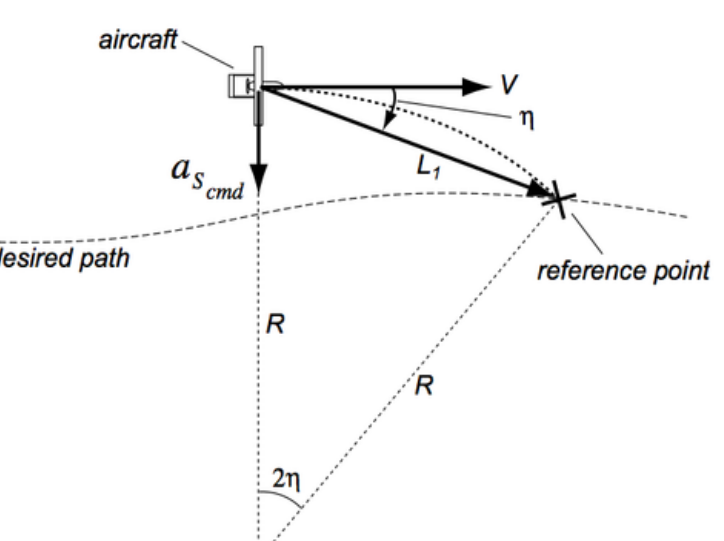
\includegraphics[width=\textwidth]{images/L1_guidance.png}
\end{minipage}
\hfill
\begin{minipage}[c]{0.4\textwidth}
    \[
\begin{array}{l}
a_s = \frac{V^2}{R} = 2\frac{V^2 \sin\eta}{L_1} \\
\phi_d = \atan\left(\frac{a_s}{g}\right)
\end{array}
\]
\end{minipage}


\colorbox[HTML]{CCFFFF}{\makebox[\textwidth-2\fboxsep][l]{\bf Total Energy Control System: }}

\begin{minipage}[c]{0.5\textwidth}
\centering
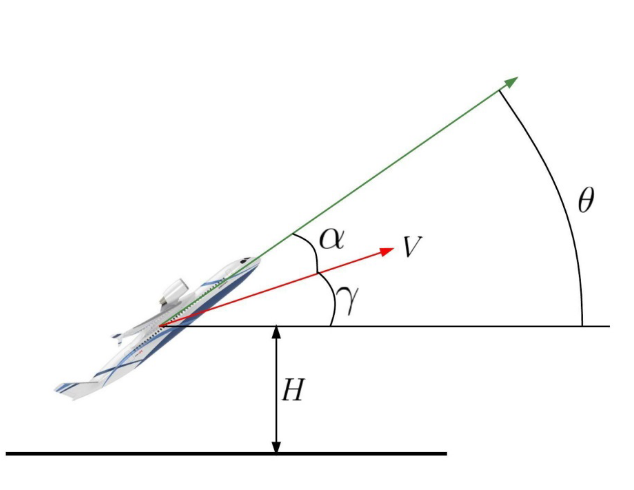
\includegraphics[width=\textwidth]{images/energy_control.png}
\end{minipage}
\hfill
\begin{minipage}[c]{0.475\textwidth}
\begin{itemize}
    \item $\begin{aligned}\dot{E}_{\text{spec}} &= \frac{\dot{E}_{\text{tot}}}{mgV} \\&= \frac{\dot{V}}{g} + \sin\gamma \\&\approx \frac{\dot{V}}{g} + \gamma\end{aligned}$
    \item $\dot{E}_{\text{dist}} = \gamma - \frac{\dot{V}}{g}$
\end{itemize}
\end{minipage}







}


%----------------------------------------------------------------
%	Fixed Wing
%----------------------------------------------------------------
\headerbox{}{name=conclusion,column=2,span=1}{
\colorbox[HTML]{CCFFFF}{\makebox[\textwidth-2\fboxsep][l]{\bf Modeling for Control(Linearized Plant): }}

\begin{itemize}\compresslist
    \item \textit{Longitudinal Plant}
   
      \textbf{Input}: $\Delta \delta_e, \Delta\delta_T$
      
      \textbf{Output}: $\Delta u, \Delta w, \Delta q,\Delta\theta$
      \begin{itemize}[label=$\circ$]\compresslist
        \item Short Period Mode $\mathbb{C}$: $\omega=5\text{rad}/s$ 
        % Include image here with \includegraphics{path/to/short-period-mode.png}
        % Example: \includegraphics[width=0.5\textwidth]{path/to/short-period-mode.png}
        \item Exchange between kinetic and potential energy: slow
        \item Phugoid Mode $\mathbb{C}$: $\omega = 0.6~\text{rad}/s$
        % Include image here with \includegraphics{path/to/phugoid_mode.png}
        \item Oscillation of angle of attack: fast
    \end{itemize}
\item \textit{Lateral Plant}

  \textbf{Input}: $\Delta \delta_a, \Delta \delta_r$
  
  \textbf{Output}: $\Delta v,\Delta p, \Delta r, \Delta\phi,\Delta\psi$
  \begin{itemize}[label=$\circ$]\compresslist
    \item Spiral Mode $\mathbb{R}$: unstable
    % Include image here with \includegraphics{path/to/spiral_mode.png}
    \item Dutch Roll Mode $\mathbb{C}$: $\omega = 5\text{rad}/s$
    % Include image here with \includegraphics{path/to/Dutch_Roll_mode.png}
    \item Roll Subsidence $\mathbb{R}$
  \end{itemize}
\end{itemize}
}

%----------------------------------------------------------------
%	Statements
%----------------------------------------------------------------
\headerbox{Statements}{name=conclusion,column=2,row=0.4}{

\colorbox[HTML]{CCFFFF}{\makebox[\textwidth-2\fboxsep][l]{\bf Kinematics: }}

\begin{itemize}\compresslist
    \item[$\times$] A homogeneous transformation $T_{\mathcal {AB}}$ from frame $\mathcal B$ to $\mathcal A$ applied to a vector only changes its representation but not the underlying $v$.
    \item[$\checkmark$] A rotation matrix $C_{\mathcal {AB}}$ between frame $\mathcal B$ to $\mathcal A$ applied to a vector only changes its representation but not the underlying $v$.
    \item[$\times$] A planar two-link robot arm has a unique solution to the inverse kinematic problem.
    \item[$\times$] For a planar two-link robot arm, the differential inverse kinematic algorithm always converges to the same solution irrespective of initial configuration.
    \item[$\times$] In floating base in 3-dimensional space there exists a choice of generalized coordinates such that the analytical and geometric orientation Jacobian are equal.
\end{itemize}

\colorbox[HTML]{CCFFFF}{\makebox[\textwidth-2\fboxsep][l]{\bf Dynamics: }}

\begin{itemize}\compresslist
    \item[$\times$] Given a perfect model, a robotic arm controlled by a PD controller with gravity compensation can achieve zero tracking error for any desired trajectory.
    \item[$\times$] When choosing a unit quaternion as part of the generalized coordinates of a free-floating rigid body in 3D space, the mass matrix must have dimensions $7\times 7$.
\end{itemize}




}

%----------------------------------------------------------------
%	Statements
%----------------------------------------------------------------
\headerbox{Statements}{name=conclusion,column=3,row=0}{

\colorbox[HTML]{CCFFFF}{\makebox[\textwidth-2\fboxsep][l]{\bf Legged Robot: }}

\begin{itemize}\compresslist
    \item[$\checkmark$] For a bipedal system with two point feet on the ground, every torque command results in a unique acceleration.
    \item[$\times$] For a bipedal system with two point feet on the ground, every constraint consistent acceleration $\dot u^*_{consistent}$ is achieved by a unique torque command.
\end{itemize}



\colorbox[HTML]{CCFFFF}{\makebox[\textwidth-2\fboxsep][l]{\bf Rotor Craft: }}

\begin{itemize}\compresslist
     \item[$\times$] A classic hexacopter (multi-rotor with 6 propellers) with all propellers spinning in the same plane is a fully actuated platform.
    \item[$\checkmark$] The yaw motion for a quadcopter is controlled by the drag moment of the propeller.
    \item[$\times$] The attitude dynamics of a quadcopter can be stabilized by a proportional controller only.
    \item[$\times$] The hub force on a rotor in forward flight results mostly due to an imbalance of the lift forces on the advancing and the retreating blade.
    \item[$\checkmark$] BEMT can be used to model propeller characteristics, where momentum theory enables solving for induced velocities.
    \item[$\times$] A swashplate has generally three degrees of freedom. One to control the cyclic pitch and two to control the collective pitch.
    \item[$\times$] A rotor in forward motion has a reverse flow region on the advancing blade.
    \item[$\times$] In a front-rear rotor configuration, the yaw motion is steered by differential drag torques of the rotors.
    \item[$\checkmark$]  According to the momentum theory, the power consumption decrease to zero  by increasing  the disc area to infinity
\end{itemize}



\colorbox[HTML]{CCFFFF}{\makebox[\textwidth-2\fboxsep][l]{\bf Fixed Wing: }}

\begin{itemize}\compresslist
    \item[$\times$] The magnitude of the GPS velocity can be used directly as an airspeed measurement
    \item[$\times$] The heading of a conventional aircraft is controlled primarily by the rudder 
    \item[$\checkmark$] Wind disturbances are typically modeled/mitigated within the guidance-
  level loops of a fixed-wing autopilot 
    \item[$\checkmark$] Minimum airspeed demand during a coordinated turn increases as the
  turning radius decreases, assuming constant angle of attach 
    \item[$\times$] in a coordinate turn, the sideslip force causes the needed centripetal acceleration
\end{itemize}
}

\end{poster}

\end{document}